% Options for packages loaded elsewhere
\PassOptionsToPackage{unicode}{hyperref}
\PassOptionsToPackage{hyphens}{url}
%
\documentclass[
]{book}
\usepackage{amsmath,amssymb}
\usepackage{iftex}
\ifPDFTeX
  \usepackage[T1]{fontenc}
  \usepackage[utf8]{inputenc}
  \usepackage{textcomp} % provide euro and other symbols
\else % if luatex or xetex
  \usepackage{unicode-math} % this also loads fontspec
  \defaultfontfeatures{Scale=MatchLowercase}
  \defaultfontfeatures[\rmfamily]{Ligatures=TeX,Scale=1}
\fi
\usepackage{lmodern}
\ifPDFTeX\else
  % xetex/luatex font selection
\fi
% Use upquote if available, for straight quotes in verbatim environments
\IfFileExists{upquote.sty}{\usepackage{upquote}}{}
\IfFileExists{microtype.sty}{% use microtype if available
  \usepackage[]{microtype}
  \UseMicrotypeSet[protrusion]{basicmath} % disable protrusion for tt fonts
}{}
\makeatletter
\@ifundefined{KOMAClassName}{% if non-KOMA class
  \IfFileExists{parskip.sty}{%
    \usepackage{parskip}
  }{% else
    \setlength{\parindent}{0pt}
    \setlength{\parskip}{6pt plus 2pt minus 1pt}}
}{% if KOMA class
  \KOMAoptions{parskip=half}}
\makeatother
\usepackage{xcolor}
\usepackage{color}
\usepackage{fancyvrb}
\newcommand{\VerbBar}{|}
\newcommand{\VERB}{\Verb[commandchars=\\\{\}]}
\DefineVerbatimEnvironment{Highlighting}{Verbatim}{commandchars=\\\{\}}
% Add ',fontsize=\small' for more characters per line
\usepackage{framed}
\definecolor{shadecolor}{RGB}{248,248,248}
\newenvironment{Shaded}{\begin{snugshade}}{\end{snugshade}}
\newcommand{\AlertTok}[1]{\textcolor[rgb]{0.94,0.16,0.16}{#1}}
\newcommand{\AnnotationTok}[1]{\textcolor[rgb]{0.56,0.35,0.01}{\textbf{\textit{#1}}}}
\newcommand{\AttributeTok}[1]{\textcolor[rgb]{0.13,0.29,0.53}{#1}}
\newcommand{\BaseNTok}[1]{\textcolor[rgb]{0.00,0.00,0.81}{#1}}
\newcommand{\BuiltInTok}[1]{#1}
\newcommand{\CharTok}[1]{\textcolor[rgb]{0.31,0.60,0.02}{#1}}
\newcommand{\CommentTok}[1]{\textcolor[rgb]{0.56,0.35,0.01}{\textit{#1}}}
\newcommand{\CommentVarTok}[1]{\textcolor[rgb]{0.56,0.35,0.01}{\textbf{\textit{#1}}}}
\newcommand{\ConstantTok}[1]{\textcolor[rgb]{0.56,0.35,0.01}{#1}}
\newcommand{\ControlFlowTok}[1]{\textcolor[rgb]{0.13,0.29,0.53}{\textbf{#1}}}
\newcommand{\DataTypeTok}[1]{\textcolor[rgb]{0.13,0.29,0.53}{#1}}
\newcommand{\DecValTok}[1]{\textcolor[rgb]{0.00,0.00,0.81}{#1}}
\newcommand{\DocumentationTok}[1]{\textcolor[rgb]{0.56,0.35,0.01}{\textbf{\textit{#1}}}}
\newcommand{\ErrorTok}[1]{\textcolor[rgb]{0.64,0.00,0.00}{\textbf{#1}}}
\newcommand{\ExtensionTok}[1]{#1}
\newcommand{\FloatTok}[1]{\textcolor[rgb]{0.00,0.00,0.81}{#1}}
\newcommand{\FunctionTok}[1]{\textcolor[rgb]{0.13,0.29,0.53}{\textbf{#1}}}
\newcommand{\ImportTok}[1]{#1}
\newcommand{\InformationTok}[1]{\textcolor[rgb]{0.56,0.35,0.01}{\textbf{\textit{#1}}}}
\newcommand{\KeywordTok}[1]{\textcolor[rgb]{0.13,0.29,0.53}{\textbf{#1}}}
\newcommand{\NormalTok}[1]{#1}
\newcommand{\OperatorTok}[1]{\textcolor[rgb]{0.81,0.36,0.00}{\textbf{#1}}}
\newcommand{\OtherTok}[1]{\textcolor[rgb]{0.56,0.35,0.01}{#1}}
\newcommand{\PreprocessorTok}[1]{\textcolor[rgb]{0.56,0.35,0.01}{\textit{#1}}}
\newcommand{\RegionMarkerTok}[1]{#1}
\newcommand{\SpecialCharTok}[1]{\textcolor[rgb]{0.81,0.36,0.00}{\textbf{#1}}}
\newcommand{\SpecialStringTok}[1]{\textcolor[rgb]{0.31,0.60,0.02}{#1}}
\newcommand{\StringTok}[1]{\textcolor[rgb]{0.31,0.60,0.02}{#1}}
\newcommand{\VariableTok}[1]{\textcolor[rgb]{0.00,0.00,0.00}{#1}}
\newcommand{\VerbatimStringTok}[1]{\textcolor[rgb]{0.31,0.60,0.02}{#1}}
\newcommand{\WarningTok}[1]{\textcolor[rgb]{0.56,0.35,0.01}{\textbf{\textit{#1}}}}
\usepackage{longtable,booktabs,array}
\usepackage{calc} % for calculating minipage widths
% Correct order of tables after \paragraph or \subparagraph
\usepackage{etoolbox}
\makeatletter
\patchcmd\longtable{\par}{\if@noskipsec\mbox{}\fi\par}{}{}
\makeatother
% Allow footnotes in longtable head/foot
\IfFileExists{footnotehyper.sty}{\usepackage{footnotehyper}}{\usepackage{footnote}}
\makesavenoteenv{longtable}
\usepackage{graphicx}
\makeatletter
\def\maxwidth{\ifdim\Gin@nat@width>\linewidth\linewidth\else\Gin@nat@width\fi}
\def\maxheight{\ifdim\Gin@nat@height>\textheight\textheight\else\Gin@nat@height\fi}
\makeatother
% Scale images if necessary, so that they will not overflow the page
% margins by default, and it is still possible to overwrite the defaults
% using explicit options in \includegraphics[width, height, ...]{}
\setkeys{Gin}{width=\maxwidth,height=\maxheight,keepaspectratio}
% Set default figure placement to htbp
\makeatletter
\def\fps@figure{htbp}
\makeatother
\setlength{\emergencystretch}{3em} % prevent overfull lines
\providecommand{\tightlist}{%
  \setlength{\itemsep}{0pt}\setlength{\parskip}{0pt}}
\setcounter{secnumdepth}{5}
\usepackage{booktabs}
\ifLuaTeX
  \usepackage{selnolig}  % disable illegal ligatures
\fi
\usepackage[]{natbib}
\bibliographystyle{apalike}
\usepackage{bookmark}
\IfFileExists{xurl.sty}{\usepackage{xurl}}{} % add URL line breaks if available
\urlstyle{same}
\hypersetup{
  pdftitle={yet another SNA coursebook},
  pdfauthor={Arthur Pecherskikh},
  hidelinks,
  pdfcreator={LaTeX via pandoc}}

\title{yet another SNA coursebook}
\author{Arthur Pecherskikh}
\date{2025-10-29}

\begin{document}
\maketitle

{
\setcounter{tocdepth}{1}
\tableofcontents
}
\chapter*{\texorpdfstring{\textbf{Intro}}{Intro}}\label{intro}
\addcontentsline{toc}{chapter}{\textbf{Intro}}

Arthur Pecherskikh (\href{aapecherskikh@eu.spb.ru}{apecherskikh@eu.spb.ru} \textbar{} \url{aapecherskikh@hse.ru})\\
\emph{last update:} 2025-10-29

The network metaphor has become a prevalent part of contemporary societies. Ideas that have been developed in the social sciences over decades are now widely accepted by the general public. We frequently discuss the importance of ``networking'', someone's ``connections'', or ``social capital''. The daily presence of social media platforms (e.g., Telegram, VK, Twitter) in our lives -- where we observe others' numbers of friends and are often surprised when two seemingly distant acquaintances turn out to be connected -- makes the subject of this course self-evident on the surface. However, the social network analysis (SNA) is much more than just a common metaphor; it is a powerful and well-formalized set of methods used to study complex real-world phenomena, from the spread of rumors or diseases (as seen recently with COVID-19) to global trade networks and the rise and fall of creativity in cultural industries.

SNA is an analysis-heavy subfield, meaning (1) it is challenging to come up with a general theory of social networks due to their diversity and complexity (viewing social reality relationally is one of the few unifying principles), and (2) it is difficult to grasp without hands-on experience with data. For these reasons, this course will focus on teaching you (1) how to develop researchable ideas and (2) how to test these ideas using available statistical software. The general goal of this course is thus to provide participants with essential insights into social networks and to equip them with the skills to analyze networks computationally.

\section*{\texorpdfstring{\textbf{About me}}{About me}}\label{about-me}
\addcontentsline{toc}{section}{\textbf{About me}}

My name is Arthur Pecherskikh, I am a second-year PhD student at European University at St.~Petersburg (sociology program) and researcher at the \href{https://ciase.ru/}{Center for Institutional Analysis of Science \& Education}. My research interests include social network analysis, sociology of science, artistic consecration, sociology of sociology, and computational text analysis.

\begin{center}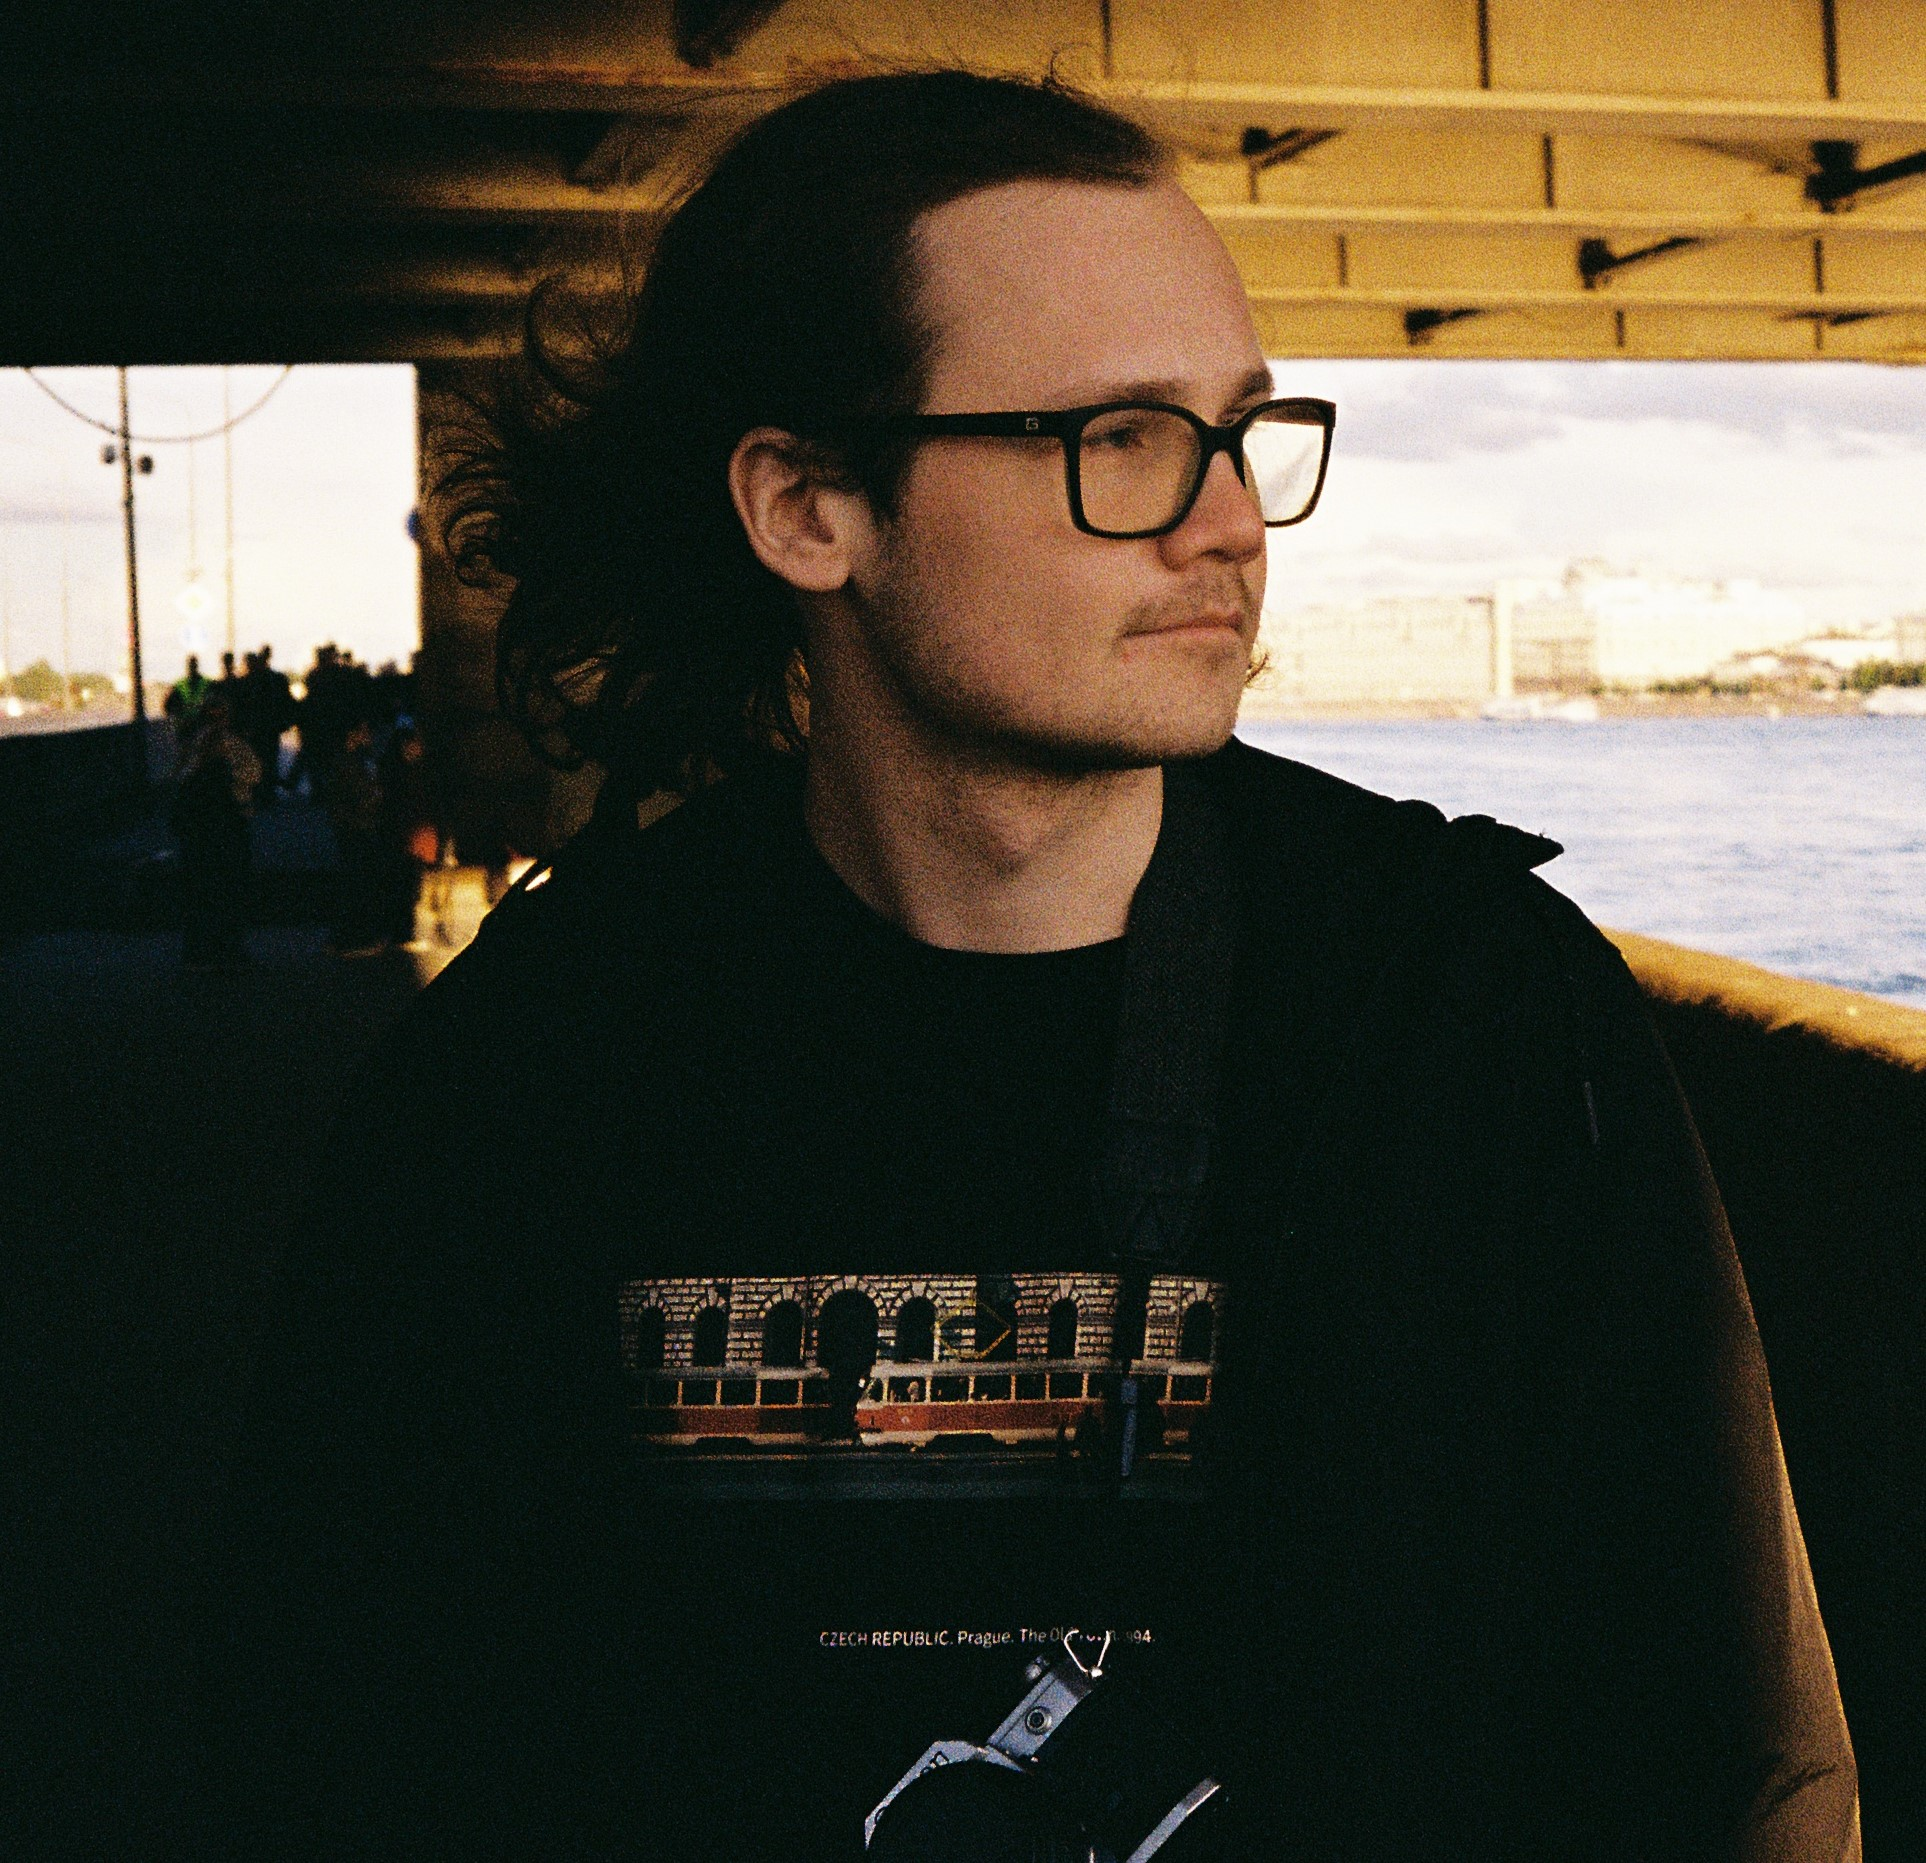
\includegraphics[width=1\linewidth]{images/arthur-pick} \end{center}

This is the second time I teach networks at the master program ``Data Analytics for Business and Economics'' (Higher School of Economics, St.~Petersburg), and the last-year course page at HSE website is available \href{https://spb.hse.ru/en/ma/data-analytics/courses/904345939.html}{here}. The organization and structure of this course have been heavily influenced by Maria Safonova eponymous lectures I took some years ago. In developing the course, I also consulted the syllabi created by Nadya Sokolova (2023), John Levi Martin (2008), Paul McLean (2021), Mark Mizruchi (2008), Chris Smith (2022), and Steve Borgatti (2004).

Whatever question about the course you have, please, contact me via corporate email (\url{aapecherskikh@hse.ru}) or telegram (my nickname is {@archibard}).

\chapter*{\texorpdfstring{\textbf{Formalities}}{Formalities}}\label{formalities}
\addcontentsline{toc}{chapter}{\textbf{Formalities}}

The course consists of six meetings held on Thursdays at 18:10 on Kantemirovskaya. Each lesson will include a lecture followed by a practical coding workshop. Students are expected to attend class, actively participate in discussions, and engage in coding activities. The content of the last meeting (12.12) is flexible and can be changed to match the students' requests.

Your mark for the course consists of:

\textbf{- homework assignments: }60\% (5 assignments in total; the average of your 3 highest scores will be used)

\textbf{- final exam:} 40\% (individual or group project)

All assignments and projects should be submitted via email to ensure timely review and feedback. The sections below outline the details of both grading components.

\section*{\texorpdfstring{\textbf{Home assignments}}{Home assignments}}\label{home-assignments}
\addcontentsline{toc}{section}{\textbf{Home assignments}}

There will be 5 homework assignments throughout the course, but only your best 3 scores will be used to calculate your final grade. This means you can choose to complete all the homework or just 3 without it affecting your final mark. For the homework component, I will simply average your 3 highest grades. However, I strongly recommend reviewing each assignment, as completing them will better prepare you for the final project.

Homework assignments are due before the start of the next class (the exact time is 18:10, Thursday, each week). If you submit an assignment within the following week, you can still earn up to 8 points.

\section*{\texorpdfstring{\textbf{Exam}}{Exam}}\label{exam}
\addcontentsline{toc}{section}{\textbf{Exam}}

The exam can be completed either individually or in groups of up to 4 students. Your task is to conduct a small research project and report your findings in a paper of approximately 4--5 pages (including visualizations, tables, and bibliography). These length guidelines are flexible, so feel free to write more or less if needed. The exam will consist of the following elements:

\textbf{1. Collect network data}

You are free to choose your context --- whether it's networks of friends, Hollywood actors, or another topic of interest. If you are working individually, you may use pre-existing datasets from GitHub or other data archives. However, ensure you don't simply copy someone else's work entirely. Replicating a study (without access to the original code) can be a good approach, though. I would not decrease the mark for analyzing already collected data, though you can get additional 2 points if you do collect the data yourself.

\textbf{2. Describe your data}

Provide a brief overview of your dataset and highlight its key aspects. Include a readable visualization of the network you are analyzing and compute and discuss its descriptive properties (e.g., density, diameter). Be sure to consider the context of your data: how ties are formed, how actors are selected, and any other relevant details.

\textbf{3. Pose research questions}

Formulate 2--3 research questions (preferably interconnected) and explain why these questions are important. If you have any hypothesEs and supporting literature, include them in your report. Note that a larger team need either more questions or questions which are difficult to work with alone.

\textbf{4. Describe your workflow}

Discuss the materials you consulted, any ideas that came to you during the course, and how long the analysis took. Include methodological considerations and reflections on the choices you made throughout the project.

\textbf{5. Present and discuss the results}

Present your findings --- for example, this could be in the form of a table with network values. However, it is important to also provide interpretations of these results, explaining what they mean in the context of your research.

Don't hesitate to explore and experiment with the tools, as the goal is to learn through hands-on experience. Feel free to change the structure (e.g., data collection and description, research questions, methodology/inspiration/etc., results) if you feel it does not align with the type of work you are doing. The project format is flexible to suit different research interests and approaches.

In an ideal scenario, you should start thinking about your final project around the second meeting. Having ideas early will allow you to benefit more from class discussions and ask questions that specifically relate to your project.

The main purpose of the exam is to assess whether you are familiar with the basic logic of network analysis and whether you can apply some of the methods covered in the course. While the quality of your analysis is important, the focus will also be on your effort, reflection, and interpretation. Even if your technical analysis is not perfect, what matters most is your understanding of the principles of network analysis and your ability to critically reflect on your process. Network analysis can be challenging, and working with real data often presents unexpected difficulties, so the evaluation will not be overly strict. The deadline for the exam report is 19th December (by the end of the day), which is one week after our final meeting.

\section*{\texorpdfstring{\textbf{Evaluation}}{Evaluation}}\label{evaluation}
\addcontentsline{toc}{section}{\textbf{Evaluation}}

The following grading criteria apply to both homework assignments and the final exam:

\textbf{- ``Excellent'' (9--10)}

The student demonstrates deep knowledge and advanced skills, exceeding the materials discussed in the class and/or incorporating additional relevant resources. Coding procedures are thoroughly commented on, all tasks are completed without errors, and the work is properly structured.

\textbf{- ``Excellent'' (8)}

The student shows a strong understanding of the topic. While minor mistakes may be present, they do not significantly affect the results or interpretations. The work is well-structured and includes detailed explanations of the analytical procedures.

\textbf{- ``Good'' (6--7)}

The student responds correctly to most tasks but may provide some misleading interpretations and/or occasional errors that affect the results and interpretations. The work is clearly structured with appropriate comments.

\textbf{- ``Satisfactory'' (4--5)}

The student addresses about half of the assigned tasks and/or makes significant errors. Results and interpretations lack depth, and the work is not detailed enough to fully explain the analysis. Formatting is unclear.

\textbf{- ``Fail'' (0--3)}

The student fails to demonstrate knowledge of the relevant topics. Most tasks are either incorrect or not completed, and interpretations are brief or missing, with little to no reference to appropriate concepts or methods.

\section*{\texorpdfstring{\textbf{Extensions and late submissions}}{Extensions and late submissions}}\label{extensions-and-late-submissions}
\addcontentsline{toc}{section}{\textbf{Extensions and late submissions}}

If you are unable to submit a homework assignment or take the exam on time due to a valid reason (e.g., illness, conference participation, or other extenuating circumstances), please notify me as soon as possible. You may receive up to 2 additional weeks to submit a homework assignment after the general deadline, and up to 1 additional week to complete the exam.

Documentation (e.g., a medical certificate) is required to confirm the reason for the delay. Please ensure to communicate any issues before the deadline whenever possible.

\section*{\texorpdfstring{\textbf{Software requirements}}{Software requirements}}\label{software-requirements}
\addcontentsline{toc}{section}{\textbf{Software requirements}}

The primary tool for this course will be R and RStudio. R offers excellent packages for social network analysis, and it arguably provides better coverage of these methods compared to Python. I will guide you through learning how to effectively use these packages.

While R is powerful for analysis, it's not the most intuitive tool for producing network visualizations. Due to that, we will explore \href{https://gephi.org/}{Gephi} during our third meeting, as it is a highly effective tool for vizualization. Additionally, I encourage you to explore online tools like \href{https://cosmograph.app/}{Cosmograph} and \href{https://graphcommons.com/}{GraphCommons} for inspiration; these platforms also allow you to create visually appealing graphs.

\chapter*{\texorpdfstring{\textbf{Course outline}}{Course outline}}\label{course-outline}
\addcontentsline{toc}{chapter}{\textbf{Course outline}}

The table below contains an approximate outline for our activities in this module. For the last meeting, we will see if there are participants who want to present a solo/group project as their exam work (and if so, they will give us a talk), or I would prepare some materials on topics not yet covered in the course.

\begin{longtable}[]{@{}
  >{\raggedright\arraybackslash}p{(\columnwidth - 4\tabcolsep) * \real{0.2381}}
  >{\raggedright\arraybackslash}p{(\columnwidth - 4\tabcolsep) * \real{0.3810}}
  >{\raggedright\arraybackslash}p{(\columnwidth - 4\tabcolsep) * \real{0.3810}}@{}}
\toprule\noalign{}
\begin{minipage}[b]{\linewidth}\raggedright
date/topic
\end{minipage} & \begin{minipage}[b]{\linewidth}\raggedright
lecture
\end{minipage} & \begin{minipage}[b]{\linewidth}\raggedright
seminar
\end{minipage} \\
\midrule\noalign{}
\endhead
\bottomrule\noalign{}
\endlastfoot
date TBA\textbf{Introduction} & The metaphor and theory behind the set of methods. Basic definitions: nodes and edges, directed and undirected ties, weighted ties. Micro / meso / macro levels of analysis. Triads \& exchange theory (briefly). A very short history of network analysis. Examples from the range of disciplines (e.g., history, political sciences, etc.). Examples of more interest for management students. & Ways to collect network data (secondary data, questionnaires, etc.). Software overview (beyond R). A very short intro to web-scraping. Data organization: matrix and edgelist. Loading data to R. \\
date TBA\textbf{Centrality measures and network positions} & Overview of the centrality measures. Degree centrality vs.~betweennesss centrality. Problems with the most common centrality measures. Brokerage and Burt's constraint. Weak ties and -- good ideas, job search, etc. & Practical session: from data loading to metrics' computation. We will work with a number of networks from various contexts (educational, corporate, criminal, and so on) to check if the observed measures of centrality are universal and to learn how to choose them correctly. Finally, we will take the network measures to run simple regression models. \\
date TBA\textbf{Topology and network structures} & Network descriptive statistics: number of ties/nodes, diameter, shortest paths, etc. Density, reciprocity, clustering coefficient. Homophily. Community detection algorithms (briefly). Core/periphery strcture. ``Small world'' networks. Cultural and organizational consequences of different structures. & Network visualizaions (R and other softwares: Gephi, Pajek, Cosmograph, etc.) and how to use them properly in storytelling. Computing network measures. Community detecton practice. Testing the empirical network structure against network compositions discussed in class. \\
date TBA\textbf{2-mode networks} & Towards the theory of n-mode networks. Affiliation networks. Network projections and the ``dual perspective''. Vizualizations and analytical tips. Dimensionality reduction techniques for 2-mode data. Examples from the American corporate elite and the company's interlocking. & Workshop on 2-mode networks. During this class, we will go through the typical workflow for the 2-mode networks and revise the previous topics (e.g., apply the community detection algorithms to the network projections or find the most important nodes in one of them). \\
date TBA\textbf{Structural equivalence} & Classical structuralist approaches to network analysis and why do we need them. Positions, blocks, roles. Network structures and blockmodeling. & Practical session on blockmodeling. We will learn these techniques by looking at networks of different relations among the company employees. We will also discuss why we might need multiple types of relations when doing social network analysis. \\
date TBA\textbf{Course overview and new directions} & Course participants may suggest the topics they are interested in for this class. My suggestions are temporal networks and/or ERGM. We can also consider a particular phenomenon (job search, corporate interlocking, etc.) or concept (negative ties, 2-mode networks, etc.) in more details. & TBA \\
\end{longtable}

\chapter*{\texorpdfstring{(PART*) \textbf{Seminars}}{(PART*) Seminars}}\label{part-seminars}
\addcontentsline{toc}{chapter}{(PART*) \textbf{Seminars}}

\chapter*{\texorpdfstring{\textbf{Seminar 1 - Intro}}{Seminar 1 - Intro}}\label{seminar-1---intro}
\addcontentsline{toc}{chapter}{\textbf{Seminar 1 - Intro}}

The notes below accompany the first lecture of the course. It might be a good idea to consult the {lecture slides} as well, as some technical details and examples are discussed there.

During today's meeting we are going to cover the very basics of doing network analysis in R. Relying on commonly used \texttt{igraph} package for data manipulation, we would learn about typical network data formats (edgelists, nodelists, and matrices) and how to convert them to (and from) typical tabular formats, and ways to manipulate and refer to edges and nodes of the constructed networks. We will also make our first attempts at analysis of the two exemplar datasets. After this session, you will be prepared for more concrete discussions of the network-related topics.

\section*{\texorpdfstring{\textbf{Libraries}}{Libraries}}\label{libraries}
\addcontentsline{toc}{section}{\textbf{Libraries}}

The main library we would rely on throughout the course is \texttt{igraph}. It provides the functions to create, visualize, and analyze network data. The complete documentation for \texttt{igraph} is available via \href{https://igraph.org/}{its official webpage} and the section devoted to the \href{https://igraph.org/r/html/1.2.6/}{R implementation}.

\begin{Shaded}
\begin{Highlighting}[]
\CommentTok{\# load missing packages:}
\CommentTok{\#install.packages("igraph")}
\CommentTok{\#install.packages("intergraph")}
\CommentTok{\#install.packages("manynet")}

\FunctionTok{library}\NormalTok{(tidyverse)    }\DocumentationTok{\#\# general framework to work in R}
\FunctionTok{library}\NormalTok{(igraph)       }\DocumentationTok{\#\# general package for network analysis}
\FunctionTok{library}\NormalTok{(intergraph)   }\DocumentationTok{\#\# convert from df to graph{-}objects and vice versa;}
                      \DocumentationTok{\#\# also helpful to convert "igraph" to "network" format}
\FunctionTok{library}\NormalTok{(manynet)      }\DocumentationTok{\#\# datasets}
\end{Highlighting}
\end{Shaded}

\section*{\texorpdfstring{\textbf{Common data structures and procedures}}{Common data structures and procedures}}\label{common-data-structures-and-procedures}
\addcontentsline{toc}{section}{\textbf{Common data structures and procedures}}

Networks are typically represented using two primary data formats. The first is an \textbf{adjacency matrix}, a square matrix where rows and columns represent nodes, and the cell values indicate the presence or weight of a tie between them. The second common format is an \textbf{edgelist}, which is a simple two-column list recording each connection as a pair of node identifiers. Often, an edgelist is accompanied by a separate \textbf{nodelist} that contains additional attributes for each node, such as names, gender, age, affiliations, etc. Matrices are efficient for dense, small networks and mathematical operations, while edgelists are more intuitive and memory-efficient for storing large, sparse networks. Altough we would not use matrices a lot, it is still important to think of such representations of your data during our further workshops (e.g., when we would discuss blockmodels).

Below is an image of the network obtained from Zachary's (1977) study (we will get to constructing such network objects and visualizations later, for now it is useful just to see this image). Here is the data description as given in the \texttt{manynet} package:

\begin{quote}
The network was observed in a university Karate club in 1977. The network describes association patterns among 34 members and maps out allegiance patterns between members and either Mr.~Hi, the instructor, or the John A. the club president after an argument about hiking the price for lessons. The allegiance of each node is listed in the obc argument which takes the value 1 if the individual sided with Mr.~Hi after the fight and 2 if the individual sided with John A.
\end{quote}

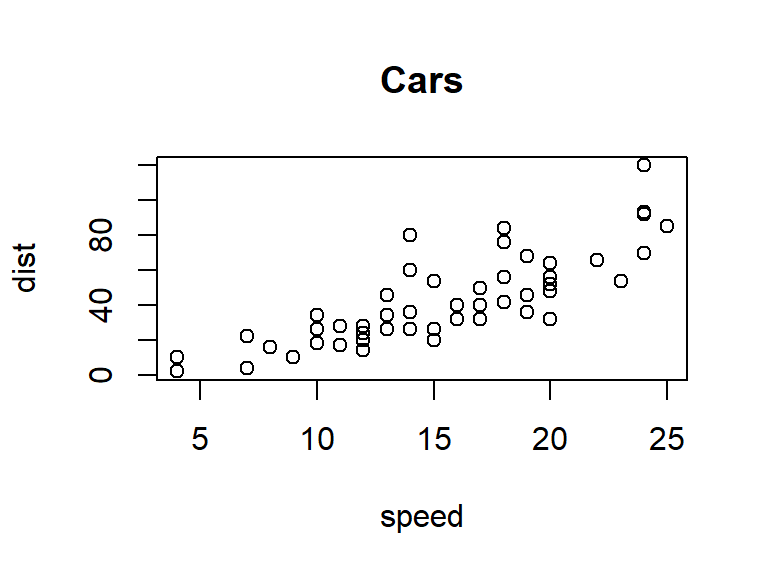
\includegraphics{chapter1_files/figure-latex/unnamed-chunk-2-1.pdf}

Now, let's look at the ways of representing this data. The \texttt{igraph} package provides simple functions to convert its network objects into standard data formats. You can transform a network to a matrix using the \texttt{as\_adjacency\_matrix()} function, which will create a square matrix representation. Each row/column here represents the person who sends the ties to the others (ties either exist, 1, or not, 0). Note that the diagonal of these matrix is filled with empty values, - it is common for network analysis that we do not want to record self-references, as they do not make sense (alhough there are cases when it is useful).

The \texttt{as\_adj()} function also works.

\begin{Shaded}
\begin{Highlighting}[]
\DocumentationTok{\#\# the object \textasciigrave{}ison\_karateka\textasciigrave{} is available via "manynet" package,}
\DocumentationTok{\#\# and it is just an "igraph" object representing a network.}
\DocumentationTok{\#\# we will discuss it below, just focus on data formats for now:}

\DocumentationTok{\#\# matrix:}
\NormalTok{ison\_karateka }\SpecialCharTok{\%\textgreater{}\%} 
  \FunctionTok{as\_adjacency\_matrix}\NormalTok{()}
\CommentTok{\#\textgreater{} 34 x 34 sparse Matrix of class "dgCMatrix"}
\CommentTok{\#\textgreater{}   [[ suppressing 34 column names \textquotesingle{}Mr Hi\textquotesingle{}, \textquotesingle{}2\textquotesingle{}, \textquotesingle{}3\textquotesingle{} ... ]]}
\CommentTok{\#\textgreater{}                                                           }
\CommentTok{\#\textgreater{} Mr Hi  . 1 1 1 1 1 1 1 1 . 1 1 1 1 . . . 1 . 1 . 1 . . . .}
\CommentTok{\#\textgreater{} 2      1 . 1 1 . . . 1 . . . . . 1 . . . 1 . 1 . 1 . . . .}
\CommentTok{\#\textgreater{} 3      1 1 . 1 . . . 1 1 1 . . . 1 . . . . . . . . . . . .}
\CommentTok{\#\textgreater{} 4      1 1 1 . . . . 1 . . . . 1 1 . . . . . . . . . . . .}
\CommentTok{\#\textgreater{} 5      1 . . . . . 1 . . . 1 . . . . . . . . . . . . . . .}
\CommentTok{\#\textgreater{} 6      1 . . . . . 1 . . . 1 . . . . . 1 . . . . . . . . .}
\CommentTok{\#\textgreater{} 7      1 . . . 1 1 . . . . . . . . . . 1 . . . . . . . . .}
\CommentTok{\#\textgreater{} 8      1 1 1 1 . . . . . . . . . . . . . . . . . . . . . .}
\CommentTok{\#\textgreater{} 9      1 . 1 . . . . . . . . . . . . . . . . . . . . . . .}
\CommentTok{\#\textgreater{} 10     . . 1 . . . . . . . . . . . . . . . . . . . . . . .}
\CommentTok{\#\textgreater{} 11     1 . . . 1 1 . . . . . . . . . . . . . . . . . . . .}
\CommentTok{\#\textgreater{} 12     1 . . . . . . . . . . . . . . . . . . . . . . . . .}
\CommentTok{\#\textgreater{} 13     1 . . 1 . . . . . . . . . . . . . . . . . . . . . .}
\CommentTok{\#\textgreater{} 14     1 1 1 1 . . . . . . . . . . . . . . . . . . . . . .}
\CommentTok{\#\textgreater{} 15     . . . . . . . . . . . . . . . . . . . . . . . . . .}
\CommentTok{\#\textgreater{} 16     . . . . . . . . . . . . . . . . . . . . . . . . . .}
\CommentTok{\#\textgreater{} 17     . . . . . 1 1 . . . . . . . . . . . . . . . . . . .}
\CommentTok{\#\textgreater{} 18     1 1 . . . . . . . . . . . . . . . . . . . . . . . .}
\CommentTok{\#\textgreater{} 19     . . . . . . . . . . . . . . . . . . . . . . . . . .}
\CommentTok{\#\textgreater{} 20     1 1 . . . . . . . . . . . . . . . . . . . . . . . .}
\CommentTok{\#\textgreater{} 21     . . . . . . . . . . . . . . . . . . . . . . . . . .}
\CommentTok{\#\textgreater{} 22     1 1 . . . . . . . . . . . . . . . . . . . . . . . .}
\CommentTok{\#\textgreater{} 23     . . . . . . . . . . . . . . . . . . . . . . . . . .}
\CommentTok{\#\textgreater{} 24     . . . . . . . . . . . . . . . . . . . . . . . . . 1}
\CommentTok{\#\textgreater{} 25     . . . . . . . . . . . . . . . . . . . . . . . . . 1}
\CommentTok{\#\textgreater{} 26     . . . . . . . . . . . . . . . . . . . . . . . 1 1 .}
\CommentTok{\#\textgreater{} 27     . . . . . . . . . . . . . . . . . . . . . . . . . .}
\CommentTok{\#\textgreater{} 28     . . 1 . . . . . . . . . . . . . . . . . . . . 1 1 .}
\CommentTok{\#\textgreater{} 29     . . 1 . . . . . . . . . . . . . . . . . . . . . . .}
\CommentTok{\#\textgreater{} 30     . . . . . . . . . . . . . . . . . . . . . . . 1 . .}
\CommentTok{\#\textgreater{} 31     . 1 . . . . . . 1 . . . . . . . . . . . . . . . . .}
\CommentTok{\#\textgreater{} 32     1 . . . . . . . . . . . . . . . . . . . . . . . 1 1}
\CommentTok{\#\textgreater{} 33     . . 1 . . . . . 1 . . . . . 1 1 . . 1 . 1 . 1 1 . .}
\CommentTok{\#\textgreater{} John A . . . . . . . . 1 1 . . . 1 1 1 . . 1 1 1 . 1 1 . .}
\CommentTok{\#\textgreater{}                       }
\CommentTok{\#\textgreater{} Mr Hi  . . . . . 1 . .}
\CommentTok{\#\textgreater{} 2      . . . . 1 . . .}
\CommentTok{\#\textgreater{} 3      . 1 1 . . . 1 .}
\CommentTok{\#\textgreater{} 4      . . . . . . . .}
\CommentTok{\#\textgreater{} 5      . . . . . . . .}
\CommentTok{\#\textgreater{} 6      . . . . . . . .}
\CommentTok{\#\textgreater{} 7      . . . . . . . .}
\CommentTok{\#\textgreater{} 8      . . . . . . . .}
\CommentTok{\#\textgreater{} 9      . . . . 1 . 1 1}
\CommentTok{\#\textgreater{} 10     . . . . . . . 1}
\CommentTok{\#\textgreater{} 11     . . . . . . . .}
\CommentTok{\#\textgreater{} 12     . . . . . . . .}
\CommentTok{\#\textgreater{} 13     . . . . . . . .}
\CommentTok{\#\textgreater{} 14     . . . . . . . 1}
\CommentTok{\#\textgreater{} 15     . . . . . . 1 1}
\CommentTok{\#\textgreater{} 16     . . . . . . 1 1}
\CommentTok{\#\textgreater{} 17     . . . . . . . .}
\CommentTok{\#\textgreater{} 18     . . . . . . . .}
\CommentTok{\#\textgreater{} 19     . . . . . . 1 1}
\CommentTok{\#\textgreater{} 20     . . . . . . . 1}
\CommentTok{\#\textgreater{} 21     . . . . . . 1 1}
\CommentTok{\#\textgreater{} 22     . . . . . . . .}
\CommentTok{\#\textgreater{} 23     . . . . . . 1 1}
\CommentTok{\#\textgreater{} 24     . 1 . 1 . . 1 1}
\CommentTok{\#\textgreater{} 25     . 1 . . . 1 . .}
\CommentTok{\#\textgreater{} 26     . . . . . 1 . .}
\CommentTok{\#\textgreater{} 27     . . . 1 . . . 1}
\CommentTok{\#\textgreater{} 28     . . . . . . . 1}
\CommentTok{\#\textgreater{} 29     . . . . . 1 . 1}
\CommentTok{\#\textgreater{} 30     1 . . . . . 1 1}
\CommentTok{\#\textgreater{} 31     . . . . . . 1 1}
\CommentTok{\#\textgreater{} 32     . . 1 . . . 1 1}
\CommentTok{\#\textgreater{} 33     . . . 1 1 1 . 1}
\CommentTok{\#\textgreater{} John A 1 1 1 1 1 1 1 .}

\CommentTok{\#ison\_karateka \%\textgreater{}\% }
\CommentTok{\#  as\_adj()}
\end{Highlighting}
\end{Shaded}

To get an edgelist, you can use the \texttt{as\_edgelist()} function, which returns a table with two columns. Variable \texttt{from} refers to the sender of the tie, and \texttt{to} refers to the tie receiver. \texttt{weight} stands for the strength of the relations among the two persons.

\begin{Shaded}
\begin{Highlighting}[]
\DocumentationTok{\#\# edgelist:}
\NormalTok{ison\_karateka }\SpecialCharTok{\%\textgreater{}\%} 
  \FunctionTok{as\_edgelist}\NormalTok{()}
\CommentTok{\#\textgreater{} \# A tibble: 78 x 3}
\CommentTok{\#\textgreater{}    from  to    weight}
\CommentTok{\#\textgreater{}    \textless{}chr\textgreater{} \textless{}chr\textgreater{}  \textless{}dbl\textgreater{}}
\CommentTok{\#\textgreater{}  1 Mr Hi 2          4}
\CommentTok{\#\textgreater{}  2 Mr Hi 3          5}
\CommentTok{\#\textgreater{}  3 2     3          6}
\CommentTok{\#\textgreater{}  4 Mr Hi 4          3}
\CommentTok{\#\textgreater{}  5 2     4          3}
\CommentTok{\#\textgreater{}  6 3     4          3}
\CommentTok{\#\textgreater{}  7 Mr Hi 5          3}
\CommentTok{\#\textgreater{}  8 Mr Hi 6          3}
\CommentTok{\#\textgreater{}  9 Mr Hi 7          3}
\CommentTok{\#\textgreater{} 10 5     7          2}
\CommentTok{\#\textgreater{} \# i 68 more rows}
\end{Highlighting}
\end{Shaded}

For the nodelist, \texttt{igraph} is of little help, as it does not have a function for retreiving the data in this format. Though, we can use the function \texttt{as\_nodelist()} from the \texttt{manynet} package. The ``name'' attribute corresponds to the ids of your nodes from the edgelist, and the ``allegiance'' is the only additional attribute associated with the nodes.

\begin{Shaded}
\begin{Highlighting}[]
\DocumentationTok{\#\# nodelist:}
\NormalTok{ison\_karateka }\SpecialCharTok{\%\textgreater{}\%} 
  \FunctionTok{as\_nodelist}\NormalTok{() }\DocumentationTok{\#\# from "manynet"}
\CommentTok{\#\textgreater{} \# A tibble: 34 x 2}
\CommentTok{\#\textgreater{}    name  allegiance}
\CommentTok{\#\textgreater{}    \textless{}chr\textgreater{}      \textless{}dbl\textgreater{}}
\CommentTok{\#\textgreater{}  1 Mr Hi          1}
\CommentTok{\#\textgreater{}  2 2              1}
\CommentTok{\#\textgreater{}  3 3              1}
\CommentTok{\#\textgreater{}  4 4              1}
\CommentTok{\#\textgreater{}  5 5              1}
\CommentTok{\#\textgreater{}  6 6              1}
\CommentTok{\#\textgreater{}  7 7              1}
\CommentTok{\#\textgreater{}  8 8              1}
\CommentTok{\#\textgreater{}  9 9              2}
\CommentTok{\#\textgreater{} 10 10             2}
\CommentTok{\#\textgreater{} \# i 24 more rows}
\end{Highlighting}
\end{Shaded}

Another package that allows converting existing ``igraph'' objects to tabular data formats is \texttt{intergraph}. It is achieved via function \texttt{asDF()} - the function returns two objects, an edgelist and a nodelist. You can refer to them using \$ sign after the function.

\begin{Shaded}
\begin{Highlighting}[]
\CommentTok{\# intergraph::asDF(ison\_karateka)}

\DocumentationTok{\#\# intergraph::asDF(ison\_karateka)$edges}
\DocumentationTok{\#\# intergraph::asDF(ison\_karateka)$vertex}
\end{Highlighting}
\end{Shaded}

Network objects in \texttt{igraph} are complex data structures that encapsulate all network information. In the chunk below, we save the network as an object in our working environment (and call it ``karate''). Using \texttt{class()} confirms the object's type (``igraph'', but you see that it is also suitable for other applications), while \texttt{str()} reveals its internal structure, which includes slots for edges, nodes, and their attributes. This specialized class (a list of vectors, in fact) is designed for efficient network computations.

\begin{Shaded}
\begin{Highlighting}[]
\DocumentationTok{\#\# load network:}
\NormalTok{karate }\OtherTok{\textless{}{-}}\NormalTok{ ison\_karateka}

\FunctionTok{class}\NormalTok{(ison\_karateka)}
\CommentTok{\#\textgreater{} [1] "mnet"      "tbl\_graph" "igraph"}
\FunctionTok{str}\NormalTok{(ison\_karateka)}
\CommentTok{\#\textgreater{} Classes \textquotesingle{}mnet\textquotesingle{}, \textquotesingle{}tbl\_graph\textquotesingle{}, \textquotesingle{}igraph\textquotesingle{}  hidden list of 10}
\CommentTok{\#\textgreater{}  $ : num 34}
\CommentTok{\#\textgreater{}  $ : logi FALSE}
\CommentTok{\#\textgreater{}  $ : num [1:78] 1 2 2 3 3 3 4 5 6 6 ...}
\CommentTok{\#\textgreater{}  $ : num [1:78] 0 0 1 0 1 2 0 0 0 4 ...}
\CommentTok{\#\textgreater{}  $ : NULL}
\CommentTok{\#\textgreater{}  $ : NULL}
\CommentTok{\#\textgreater{}  $ : NULL}
\CommentTok{\#\textgreater{}  $ : NULL}
\CommentTok{\#\textgreater{}  $ :List of 4}
\CommentTok{\#\textgreater{}   ..$ : num [1:3] 1 0 1}
\CommentTok{\#\textgreater{}   ..$ :List of 4}
\CommentTok{\#\textgreater{}   .. ..$ name : chr "Zachary\textquotesingle{}s karate club network"}
\CommentTok{\#\textgreater{}   .. ..$ nodes: chr "club members"}
\CommentTok{\#\textgreater{}   .. ..$ ties : chr "association"}
\CommentTok{\#\textgreater{}   .. ..$ year : num 1977}
\CommentTok{\#\textgreater{}   ..$ :List of 2}
\CommentTok{\#\textgreater{}   .. ..$ name      : chr [1:34] "Mr Hi" "2" "3" "4" ...}
\CommentTok{\#\textgreater{}   .. ..$ allegiance: num [1:34] 1 1 1 1 1 1 1 1 2 2 ...}
\CommentTok{\#\textgreater{}   ..$ :List of 1}
\CommentTok{\#\textgreater{}   .. ..$ weight: num [1:78] 4 5 6 3 3 3 3 3 3 2 ...}
\CommentTok{\#\textgreater{}  $ :\textless{}environment: 0x000001b546d1a550\textgreater{} }
\CommentTok{\#\textgreater{}  {-} attr(*, "active")= chr "nodes"}
\end{Highlighting}
\end{Shaded}

Next, we use the aforementioned \texttt{asDF()} function to deconstruct a network object into two standard data frames: one for edges and one for nodes. You can re-assemble these data frames into a new igraph object using the \texttt{graph\_from\_data\_frame()} function from \texttt{igraph}.

\begin{Shaded}
\begin{Highlighting}[]
\DocumentationTok{\#\# convert to data frames}
\NormalTok{karate\_edges }\OtherTok{\textless{}{-}}\NormalTok{ (karate }\SpecialCharTok{\%\textgreater{}\%}
  \FunctionTok{asDF}\NormalTok{())}\SpecialCharTok{$}\NormalTok{edge}

\NormalTok{karate\_nodes }\OtherTok{\textless{}{-}}\NormalTok{ (karate }\SpecialCharTok{\%\textgreater{}\%}
  \FunctionTok{asDF}\NormalTok{())}\SpecialCharTok{$}\NormalTok{vertex}

\DocumentationTok{\#\# igraph output after graph creation:}
\NormalTok{karate\_recreated }\OtherTok{\textless{}{-}}\NormalTok{ karate\_edges }\SpecialCharTok{\%\textgreater{}\%} 
  \FunctionTok{graph\_from\_data\_frame}\NormalTok{(}\AttributeTok{directed =}\NormalTok{ T)}

\DocumentationTok{\#\# class(karate\_recreated)}
\DocumentationTok{\#\# now, as it is pure igraph, network is "printed" in a standard igraph{-}way:}

\NormalTok{karate\_recreated}
\CommentTok{\#\textgreater{} IGRAPH d603306 DNW{-} 34 78 {-}{-} }
\CommentTok{\#\textgreater{} + attr: name (v/c), weight (e/n)}
\CommentTok{\#\textgreater{} + edges from d603306 (vertex names):}
\CommentTok{\#\textgreater{}  [1] 1 {-}\textgreater{}2  1 {-}\textgreater{}3  2 {-}\textgreater{}3  1 {-}\textgreater{}4  2 {-}\textgreater{}4  3 {-}\textgreater{}4  1 {-}\textgreater{}5  1 {-}\textgreater{}6 }
\CommentTok{\#\textgreater{}  [9] 1 {-}\textgreater{}7  5 {-}\textgreater{}7  6 {-}\textgreater{}7  1 {-}\textgreater{}8  2 {-}\textgreater{}8  3 {-}\textgreater{}8  4 {-}\textgreater{}8  1 {-}\textgreater{}9 }
\CommentTok{\#\textgreater{} [17] 3 {-}\textgreater{}9  3 {-}\textgreater{}10 1 {-}\textgreater{}11 5 {-}\textgreater{}11 6 {-}\textgreater{}11 1 {-}\textgreater{}12 1 {-}\textgreater{}13 4 {-}\textgreater{}13}
\CommentTok{\#\textgreater{} [25] 1 {-}\textgreater{}14 2 {-}\textgreater{}14 3 {-}\textgreater{}14 4 {-}\textgreater{}14 6 {-}\textgreater{}17 7 {-}\textgreater{}17 1 {-}\textgreater{}18 2 {-}\textgreater{}18}
\CommentTok{\#\textgreater{} [33] 1 {-}\textgreater{}20 2 {-}\textgreater{}20 1 {-}\textgreater{}22 2 {-}\textgreater{}22 24{-}\textgreater{}26 25{-}\textgreater{}26 3 {-}\textgreater{}28 24{-}\textgreater{}28}
\CommentTok{\#\textgreater{} [41] 25{-}\textgreater{}28 3 {-}\textgreater{}29 24{-}\textgreater{}30 27{-}\textgreater{}30 2 {-}\textgreater{}31 9 {-}\textgreater{}31 1 {-}\textgreater{}32 25{-}\textgreater{}32}
\CommentTok{\#\textgreater{} [49] 26{-}\textgreater{}32 29{-}\textgreater{}32 3 {-}\textgreater{}33 9 {-}\textgreater{}33 15{-}\textgreater{}33 16{-}\textgreater{}33 19{-}\textgreater{}33 21{-}\textgreater{}33}
\CommentTok{\#\textgreater{} [57] 23{-}\textgreater{}33 24{-}\textgreater{}33 30{-}\textgreater{}33 31{-}\textgreater{}33 32{-}\textgreater{}33 9 {-}\textgreater{}34 10{-}\textgreater{}34 14{-}\textgreater{}34}
\CommentTok{\#\textgreater{} + ... omitted several edges}
\end{Highlighting}
\end{Shaded}

The critical argument of \texttt{graph\_from\_data\_frame()} is ``vertices='', which allows you to provide the nodelist, ensuring that all node attributes are correctly reinstated into the new network object:

\begin{Shaded}
\begin{Highlighting}[]
\DocumentationTok{\#\# add vertices info:}
\NormalTok{karate\_recreated }\OtherTok{\textless{}{-}}\NormalTok{ karate\_edges }\SpecialCharTok{\%\textgreater{}\%} 
  \FunctionTok{graph\_from\_data\_frame}\NormalTok{(}\AttributeTok{directed =}\NormalTok{ T,}
                        \AttributeTok{vertices =}\NormalTok{ karate\_nodes)}

\NormalTok{karate\_recreated}
\CommentTok{\#\textgreater{} IGRAPH d606884 DNW{-} 34 78 {-}{-} }
\CommentTok{\#\textgreater{} + attr: name (v/c), allegiance (v/n), weight (e/n)}
\CommentTok{\#\textgreater{} + edges from d606884 (vertex names):}
\CommentTok{\#\textgreater{}  [1] Mr Hi{-}\textgreater{}2  Mr Hi{-}\textgreater{}3  2    {-}\textgreater{}3  Mr Hi{-}\textgreater{}4  2    {-}\textgreater{}4 }
\CommentTok{\#\textgreater{}  [6] 3    {-}\textgreater{}4  Mr Hi{-}\textgreater{}5  Mr Hi{-}\textgreater{}6  Mr Hi{-}\textgreater{}7  5    {-}\textgreater{}7 }
\CommentTok{\#\textgreater{} [11] 6    {-}\textgreater{}7  Mr Hi{-}\textgreater{}8  2    {-}\textgreater{}8  3    {-}\textgreater{}8  4    {-}\textgreater{}8 }
\CommentTok{\#\textgreater{} [16] Mr Hi{-}\textgreater{}9  3    {-}\textgreater{}9  3    {-}\textgreater{}10 Mr Hi{-}\textgreater{}11 5    {-}\textgreater{}11}
\CommentTok{\#\textgreater{} [21] 6    {-}\textgreater{}11 Mr Hi{-}\textgreater{}12 Mr Hi{-}\textgreater{}13 4    {-}\textgreater{}13 Mr Hi{-}\textgreater{}14}
\CommentTok{\#\textgreater{} [26] 2    {-}\textgreater{}14 3    {-}\textgreater{}14 4    {-}\textgreater{}14 6    {-}\textgreater{}17 7    {-}\textgreater{}17}
\CommentTok{\#\textgreater{} [31] Mr Hi{-}\textgreater{}18 2    {-}\textgreater{}18 Mr Hi{-}\textgreater{}20 2    {-}\textgreater{}20 Mr Hi{-}\textgreater{}22}
\CommentTok{\#\textgreater{} [36] 2    {-}\textgreater{}22 24   {-}\textgreater{}26 25   {-}\textgreater{}26 3    {-}\textgreater{}28 24   {-}\textgreater{}28}
\CommentTok{\#\textgreater{} + ... omitted several edges}
\end{Highlighting}
\end{Shaded}

You can directly access the sets of edges and vertices within a network using the \texttt{E()} and \texttt{V()} functions, respectively. These functions are primarily used to assign or query attributes associated with the network's elements. For example, the syntax \texttt{\{r\}V(g)\$attribute\ \textless{}-\ values} is the standard way to add a new vertex attribute to a network ``g''. In the next chunk, we assign random values to the ``strength'' attribute:

\begin{Shaded}
\begin{Highlighting}[]
\DocumentationTok{\#\# referring to:}
\FunctionTok{E}\NormalTok{(karate) }\DocumentationTok{\#\# edges}
\CommentTok{\#\textgreater{} + 78/78 edges from 9e17774 (vertex names):}
\CommentTok{\#\textgreater{}  [1] Mr Hi{-}{-}2  Mr Hi{-}{-}3  2    {-}{-}3  Mr Hi{-}{-}4  2    {-}{-}4 }
\CommentTok{\#\textgreater{}  [6] 3    {-}{-}4  Mr Hi{-}{-}5  Mr Hi{-}{-}6  Mr Hi{-}{-}7  5    {-}{-}7 }
\CommentTok{\#\textgreater{} [11] 6    {-}{-}7  Mr Hi{-}{-}8  2    {-}{-}8  3    {-}{-}8  4    {-}{-}8 }
\CommentTok{\#\textgreater{} [16] Mr Hi{-}{-}9  3    {-}{-}9  3    {-}{-}10 Mr Hi{-}{-}11 5    {-}{-}11}
\CommentTok{\#\textgreater{} [21] 6    {-}{-}11 Mr Hi{-}{-}12 Mr Hi{-}{-}13 4    {-}{-}13 Mr Hi{-}{-}14}
\CommentTok{\#\textgreater{} [26] 2    {-}{-}14 3    {-}{-}14 4    {-}{-}14 6    {-}{-}17 7    {-}{-}17}
\CommentTok{\#\textgreater{} [31] Mr Hi{-}{-}18 2    {-}{-}18 Mr Hi{-}{-}20 2    {-}{-}20 Mr Hi{-}{-}22}
\CommentTok{\#\textgreater{} [36] 2    {-}{-}22 24   {-}{-}26 25   {-}{-}26 3    {-}{-}28 24   {-}{-}28}
\CommentTok{\#\textgreater{} [41] 25   {-}{-}28 3    {-}{-}29 24   {-}{-}30 27   {-}{-}30 2    {-}{-}31}
\CommentTok{\#\textgreater{} [46] 9    {-}{-}31 Mr Hi{-}{-}32 25   {-}{-}32 26   {-}{-}32 29   {-}{-}32}
\CommentTok{\#\textgreater{} + ... omitted several edges}
\FunctionTok{V}\NormalTok{(karate) }\DocumentationTok{\#\# nodes}
\CommentTok{\#\textgreater{} + 34/34 vertices, named, from 9e17774:}
\CommentTok{\#\textgreater{}  [1] Mr Hi  2      3      4      5      6      7      8     }
\CommentTok{\#\textgreater{}  [9] 9      10     11     12     13     14     15     16    }
\CommentTok{\#\textgreater{} [17] 17     18     19     20     21     22     23     24    }
\CommentTok{\#\textgreater{} [25] 25     26     27     28     29     30     31     32    }
\CommentTok{\#\textgreater{} [33] 33     John A}

\DocumentationTok{\#\# assign random values:}
\FunctionTok{set.seed}\NormalTok{(}\DecValTok{42}\NormalTok{) }\DocumentationTok{\#\# reproducibility}
\FunctionTok{V}\NormalTok{(karate)}\SpecialCharTok{$}\NormalTok{strength }\OtherTok{=} \FunctionTok{sample}\NormalTok{(}\FunctionTok{c}\NormalTok{(}\DecValTok{1}\SpecialCharTok{:}\DecValTok{100}\NormalTok{), }\DecValTok{34}\NormalTok{)}
\end{Highlighting}
\end{Shaded}

The command \texttt{plot()} generates the most basic network visualization. It uses ``igraph''\,'s default settings to render the graph, which provides a quick, unmodified view of the network structure. This is useful for an immediate visual inspection but offers no customization. The output always includes node labels and a layout determined by a built-in algorithm. Note that for large network objects, I might take time to draw such pictures, and it is probably recommended to move to specialized packages or softwares like Gephi (we would talk about it specifically and network visualizations in general during our third meeting).

\begin{Shaded}
\begin{Highlighting}[]
\DocumentationTok{\#\# include this to keep the nodes\textquotesingle{} positions stable}
\DocumentationTok{\#\# when running it for the second time}
\FunctionTok{set.seed}\NormalTok{(}\DecValTok{42}\NormalTok{) }

\NormalTok{karate }\SpecialCharTok{\%\textgreater{}\%} 
  \FunctionTok{plot}\NormalTok{()}
\end{Highlighting}
\end{Shaded}

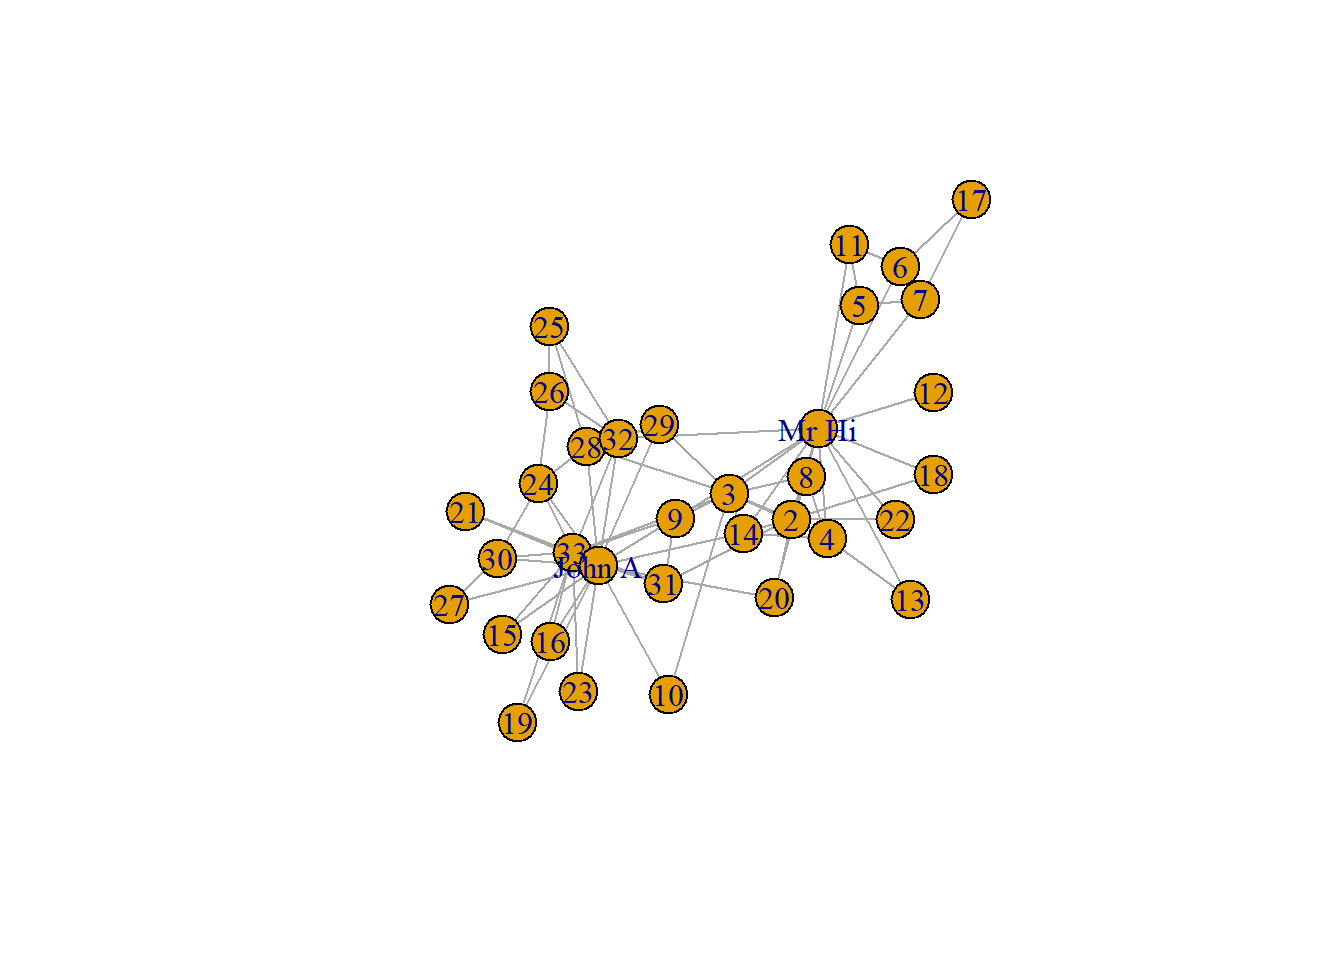
\includegraphics{chapter1_files/figure-latex/unnamed-chunk-11-1.pdf}

The next piece of code demonstrates how to customize the plot by overriding default arguments within the \texttt{plot()} function. Here, node labels are removed (``vertex.label = NA''), and all nodes are given a uniform color (via ``vertex.color'') and size (via ``vertex.size''). In my opinion, even these changes improve on the previous viz a lot.

\begin{Shaded}
\begin{Highlighting}[]
\FunctionTok{set.seed}\NormalTok{(}\DecValTok{42}\NormalTok{) }

\NormalTok{karate }\SpecialCharTok{\%\textgreater{}\%} 
  \FunctionTok{plot}\NormalTok{(}\AttributeTok{vertex.label =} \ConstantTok{NA}\NormalTok{,}
       \AttributeTok{vertex.color =} \StringTok{"coral1"}\NormalTok{,}
       \AttributeTok{vertex.size =} \DecValTok{11}\NormalTok{)}
\end{Highlighting}
\end{Shaded}

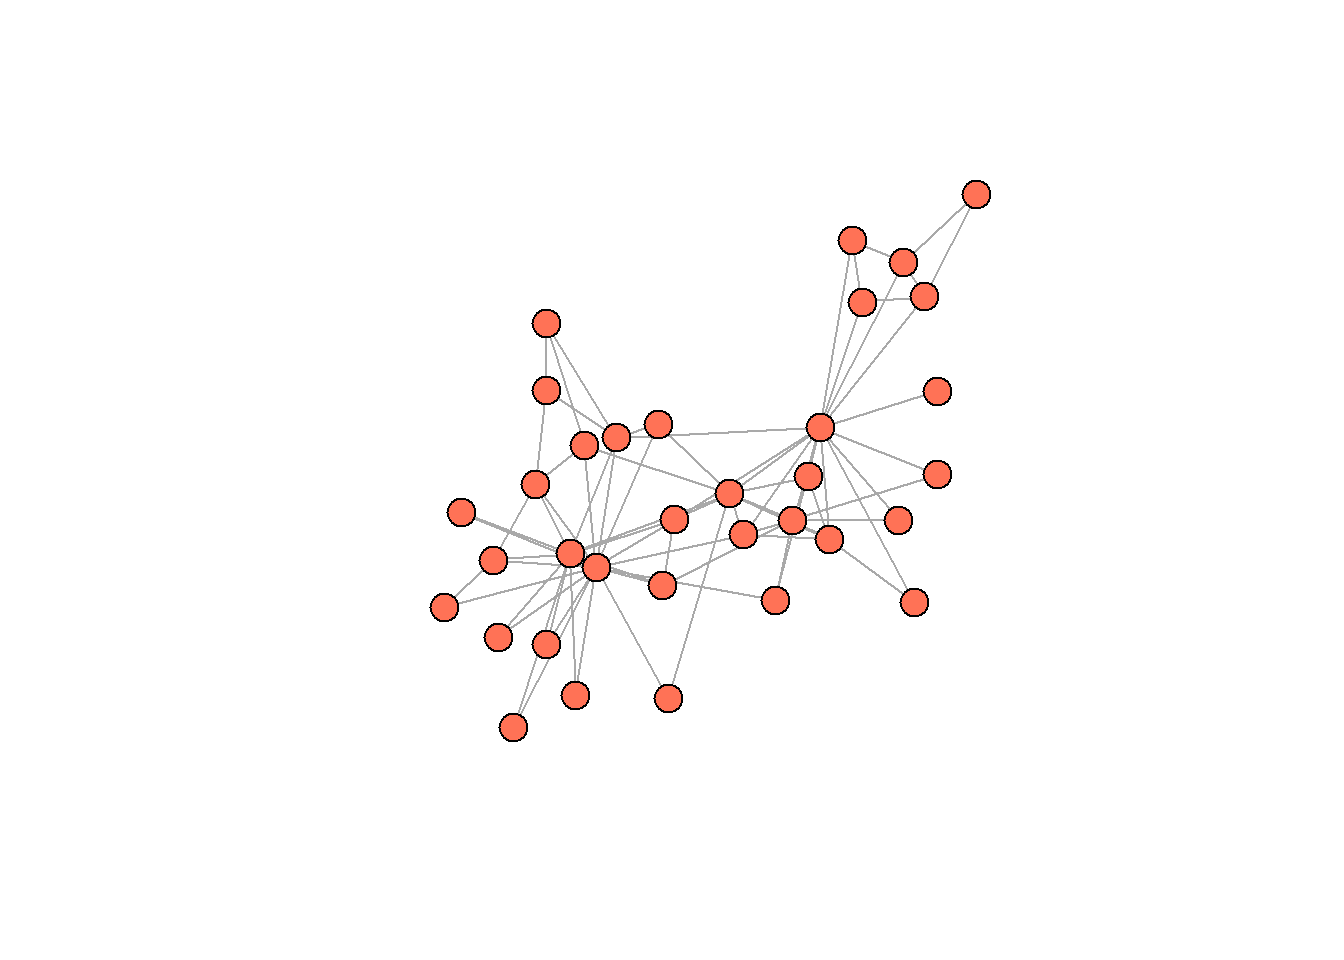
\includegraphics{chapter1_files/figure-latex/unnamed-chunk-12-1.pdf}

We can proceed to even more complex request to \texttt{plot()} function, and refer to nodes' (or edges!) attributes which are already ``in'' our ``igraph'' object. The syntax is somewhat bizarre, but you will get used to it. The idea is to use \texttt{V()} and \texttt{E()} functions to refer to either vertices (nodes) or edges from a given network, and then, using \$ sign, refer to specific attributes. In the code below, the node size is scaled based on the ``strength'' attribute (we randomly assigned these values earlier), and node color is conditionally assigned based on the ``allegiance'' attribute.

Visualizations are super important in network analysis. This steps transform the plot from a simple structural diagram into a rich visual analysis tool.

\begin{Shaded}
\begin{Highlighting}[]
\FunctionTok{set.seed}\NormalTok{(}\DecValTok{42}\NormalTok{)}

\CommentTok{\#V(karate)$strength = sample(c(1:100), 34) \#\# attribute construction}

\NormalTok{karate }\SpecialCharTok{\%\textgreater{}\%} 
  \FunctionTok{plot}\NormalTok{(}\AttributeTok{vertex.label =} \ConstantTok{NA}\NormalTok{,}
       
       \DocumentationTok{\#\# randeom strength, assigned earlier,}
       \DocumentationTok{\#\#  we divide values by 5 to get better picture:}
       \AttributeTok{vertex.size =} \FunctionTok{V}\NormalTok{(karate)}\SpecialCharTok{$}\NormalTok{strength}\SpecialCharTok{/}\DecValTok{5}\NormalTok{,}
       
       \DocumentationTok{\#\# conflict sides:}
       \AttributeTok{vertex.color =} \FunctionTok{ifelse}\NormalTok{(}\FunctionTok{V}\NormalTok{(karate)}\SpecialCharTok{$}\NormalTok{allegiance }\SpecialCharTok{==} \DecValTok{1}\NormalTok{,}
                             \StringTok{"coral1"}\NormalTok{,}
                             \StringTok{"black"}\NormalTok{),}
       
       \AttributeTok{edge.color =} \StringTok{"black"}\NormalTok{)}
\end{Highlighting}
\end{Shaded}

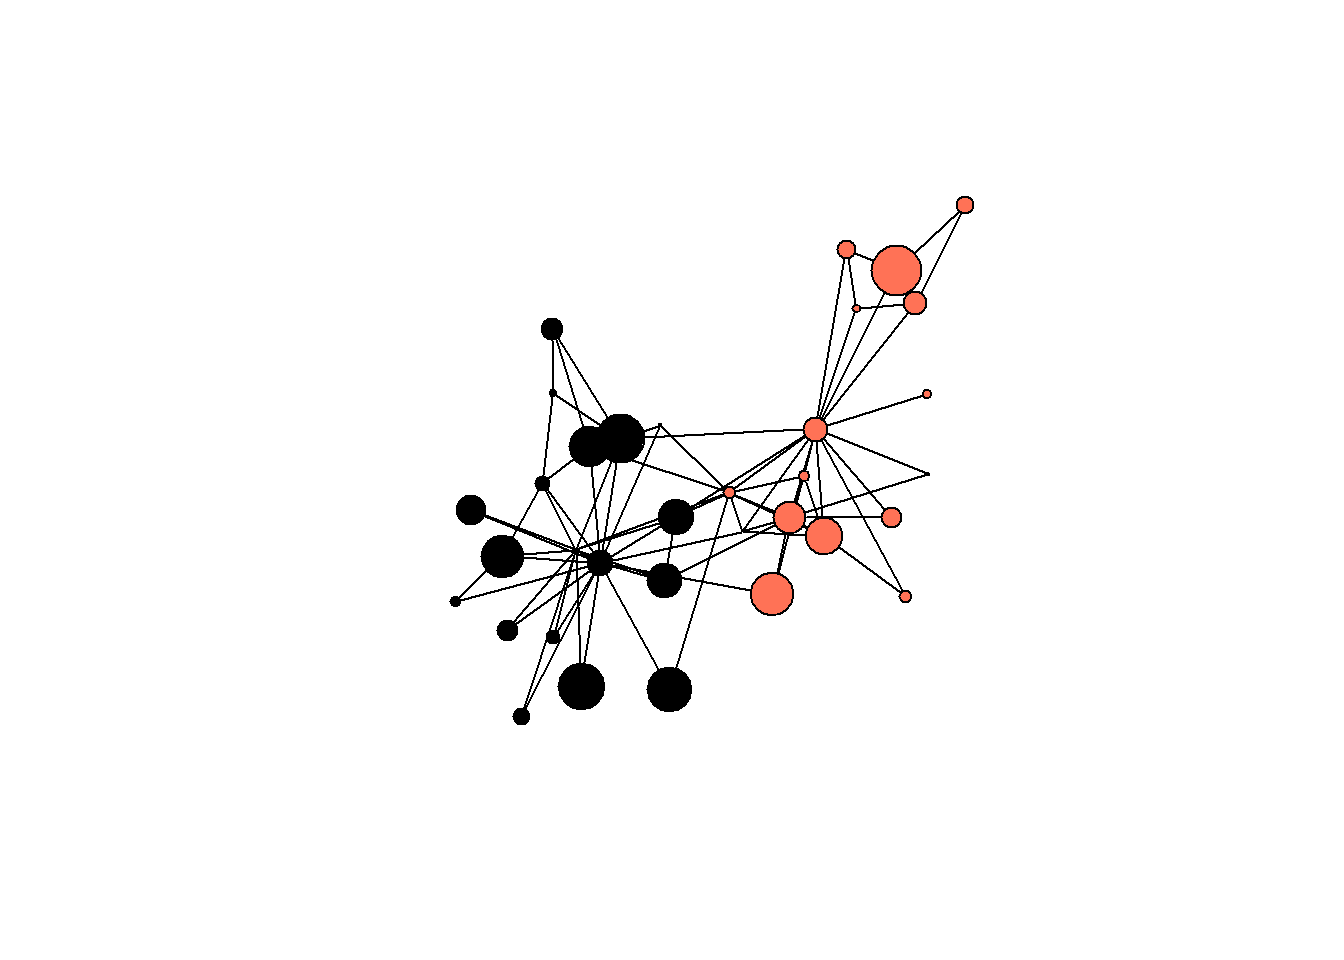
\includegraphics{chapter1_files/figure-latex/unnamed-chunk-13-1.pdf}

Here is an example of an attribute which is not random and derived exactly from network structure. This code calculates the so called degree centrality, a measure which counts the number of connections each node has (we will cover this in more details next time). The \texttt{degree()} function from \texttt{igraph} computes this, and the result is stored directly as a new vertex attribute (\texttt{V(karate)\$degree}), permanently attaching this metric to each node in the network object:

\begin{Shaded}
\begin{Highlighting}[]
\FunctionTok{V}\NormalTok{(karate)}\SpecialCharTok{$}\NormalTok{degree }\OtherTok{=}\NormalTok{ igraph}\SpecialCharTok{::}\FunctionTok{degree}\NormalTok{(karate, }\AttributeTok{mode =} \StringTok{"in"}\NormalTok{)}

\NormalTok{(}\FunctionTok{asDF}\NormalTok{(karate))}\SpecialCharTok{$}\NormalTok{vertex }\SpecialCharTok{\%\textgreater{}\%} 
  \FunctionTok{head}\NormalTok{()}
\CommentTok{\#\textgreater{}   intergraph\_id  name allegiance strength degree}
\CommentTok{\#\textgreater{} 1             1 Mr Hi          1       49     16}
\CommentTok{\#\textgreater{} 2             2     2          1       65      9}
\CommentTok{\#\textgreater{} 3             3     3          1       25     10}
\CommentTok{\#\textgreater{} 4             4     4          1       74      6}
\CommentTok{\#\textgreater{} 5             5     5          1       18      3}
\CommentTok{\#\textgreater{} 6             6     6          1      100      4}
\end{Highlighting}
\end{Shaded}

We now can work with these values in a more typical way. For example, we can plot a histogram of the degree values, which reveals the overall connectivity pattern within the network. This sort of visualizations shows the frequency of different degree levels, allowing you to see if the network is centralized around a few highly connected nodes or if connections are more evenly distributed among the participants. The former is the case for our network.

\begin{Shaded}
\begin{Highlighting}[]
\NormalTok{(}\FunctionTok{asDF}\NormalTok{(karate))}\SpecialCharTok{$}\NormalTok{vertex }\SpecialCharTok{\%\textgreater{}\%} \DocumentationTok{\#\# get the data}
  
  \FunctionTok{ggplot}\NormalTok{(}\FunctionTok{aes}\NormalTok{(degree)) }\SpecialCharTok{+} \DocumentationTok{\#\# standard ggplot2 routine}
  \FunctionTok{geom\_histogram}\NormalTok{() }\SpecialCharTok{+}
  \FunctionTok{theme\_minimal}\NormalTok{() }\SpecialCharTok{+}
  \FunctionTok{scale\_x\_continuous}\NormalTok{(}\AttributeTok{breaks =} \FunctionTok{seq}\NormalTok{(}\DecValTok{0}\NormalTok{, }\DecValTok{17}\NormalTok{, }\DecValTok{1}\NormalTok{)) }\SpecialCharTok{+}
  \FunctionTok{labs}\NormalTok{(}\AttributeTok{title =} \StringTok{"degree centrality distribution in karate network"}\NormalTok{,}
       \AttributeTok{y =} \StringTok{"\# of karate students"}\NormalTok{) }\SpecialCharTok{+}
  \FunctionTok{theme}\NormalTok{(}\AttributeTok{plot.title =} \FunctionTok{element\_text}\NormalTok{(}\AttributeTok{face=}\StringTok{"bold"}\NormalTok{))}
\CommentTok{\#\textgreater{} \textasciigrave{}stat\_bin()\textasciigrave{} using \textasciigrave{}bins = 30\textasciigrave{}. Pick better value}
\CommentTok{\#\textgreater{} \textasciigrave{}binwidth\textasciigrave{}.}
\end{Highlighting}
\end{Shaded}

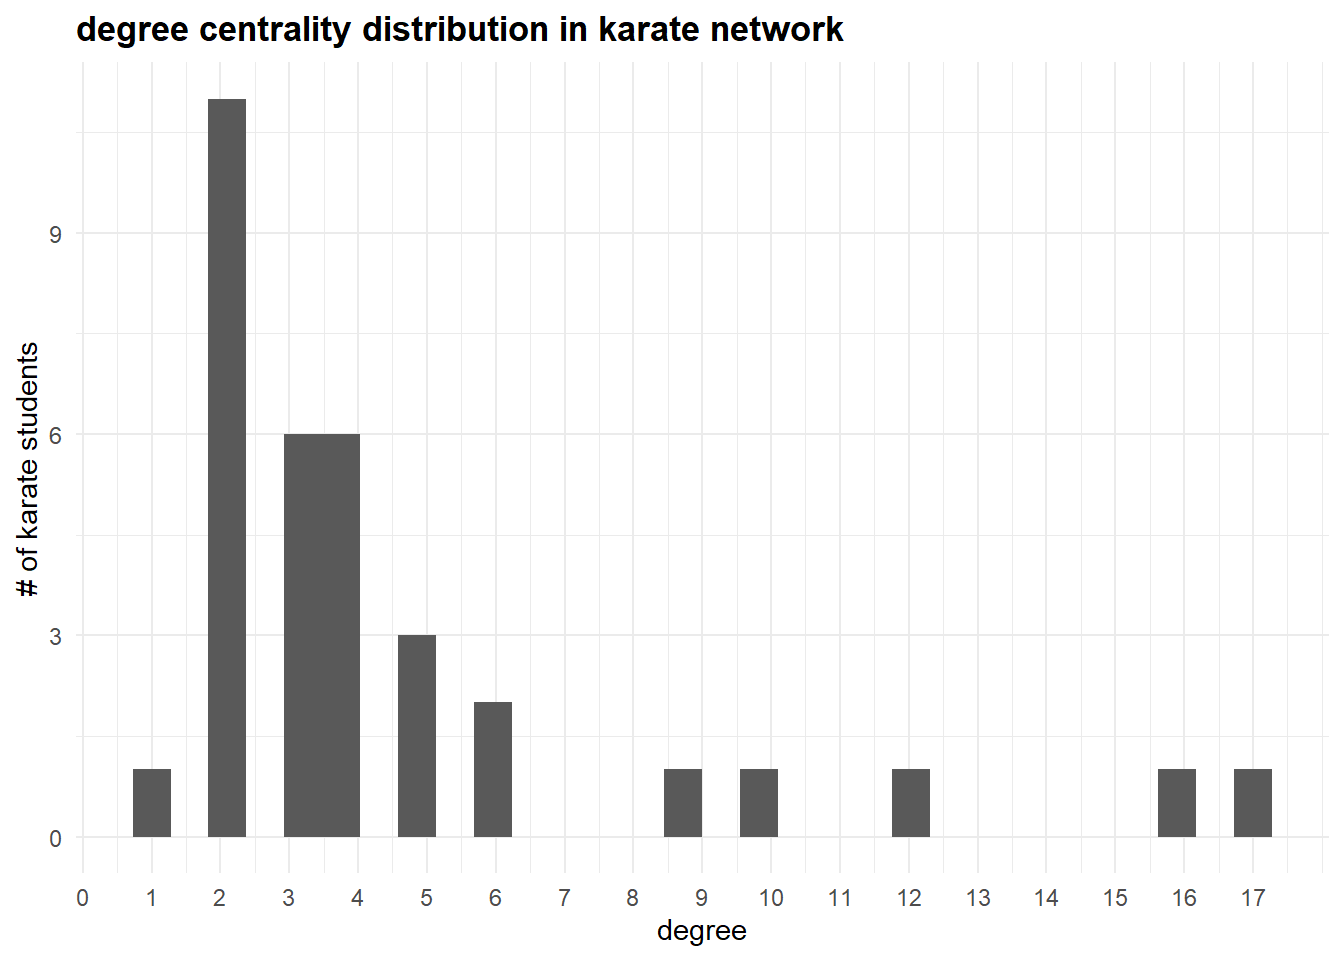
\includegraphics{chapter1_files/figure-latex/unnamed-chunk-15-1.pdf}

By grouping the nodes by their ``allegiance'' attribute, we can calculate summary statistics like the mean degree for each group (remember, ``strength'' is a made-up variable):

\begin{Shaded}
\begin{Highlighting}[]
\NormalTok{(}\FunctionTok{asDF}\NormalTok{(karate))}\SpecialCharTok{$}\NormalTok{vertex }\SpecialCharTok{\%\textgreater{}\%} 
  \FunctionTok{group\_by}\NormalTok{(allegiance) }\SpecialCharTok{\%\textgreater{}\%} 
  \FunctionTok{summarise}\NormalTok{(}\AttributeTok{mean\_degree =} \FunctionTok{round}\NormalTok{(}\FunctionTok{mean}\NormalTok{(degree),}\DecValTok{2}\NormalTok{),}
            \AttributeTok{mean\_strength =} \FunctionTok{round}\NormalTok{(}\FunctionTok{mean}\NormalTok{(strength),}\DecValTok{2}\NormalTok{))}
\CommentTok{\#\textgreater{} \# A tibble: 2 x 3}
\CommentTok{\#\textgreater{}   allegiance mean\_degree mean\_strength}
\CommentTok{\#\textgreater{}        \textless{}dbl\textgreater{}       \textless{}dbl\textgreater{}         \textless{}dbl\textgreater{}}
\CommentTok{\#\textgreater{} 1          1        4.75          41.1}
\CommentTok{\#\textgreater{} 2          2        4.44          50.7}
\end{Highlighting}
\end{Shaded}

The accompanying boxplot provides a visual comparison of the distribution of degree centrality within each group, highlighting differences in their connection patterns and allowing us to see which group's members are more central in the network:

\begin{Shaded}
\begin{Highlighting}[]
\NormalTok{(}\FunctionTok{asDF}\NormalTok{(karate))}\SpecialCharTok{$}\NormalTok{vertex }\SpecialCharTok{\%\textgreater{}\%}
  \FunctionTok{mutate}\NormalTok{(}\AttributeTok{allegiance =} \FunctionTok{as.character}\NormalTok{(allegiance)) }\SpecialCharTok{\%\textgreater{}\%}
  
  \FunctionTok{mutate}\NormalTok{(}\AttributeTok{caption =} \FunctionTok{ifelse}\NormalTok{(name }\SpecialCharTok{\%in\%} \FunctionTok{c}\NormalTok{(}\StringTok{"Mr Hi"}\NormalTok{, }\StringTok{"John A"}\NormalTok{),}
                          \FunctionTok{str\_c}\NormalTok{(}\StringTok{"}\SpecialCharTok{\textbackslash{}n}\StringTok{"}\NormalTok{, name),}
                          \StringTok{""}\NormalTok{)) }\SpecialCharTok{\%\textgreater{}\%} 
  
  \FunctionTok{ggplot}\NormalTok{(}\FunctionTok{aes}\NormalTok{(allegiance, degree)) }\SpecialCharTok{+}
  \FunctionTok{geom\_boxplot}\NormalTok{() }\SpecialCharTok{+}
  \CommentTok{\#geom\_jitter() +}
  \FunctionTok{theme\_minimal}\NormalTok{() }\SpecialCharTok{+}
  \FunctionTok{scale\_x\_discrete}\NormalTok{(}\AttributeTok{labels =} \FunctionTok{c}\NormalTok{(}\StringTok{"Mr. Hi group"}\NormalTok{, }\StringTok{"John A group"}\NormalTok{)) }\SpecialCharTok{+}
  \FunctionTok{labs}\NormalTok{(}\AttributeTok{title =} \StringTok{"degree centrality distribution in karate network"}\NormalTok{,}
       \AttributeTok{y =} \StringTok{"degree"}\NormalTok{,}
       \AttributeTok{x =} \StringTok{""}\NormalTok{) }\SpecialCharTok{+}
  \FunctionTok{theme}\NormalTok{(}\AttributeTok{plot.title =} \FunctionTok{element\_text}\NormalTok{(}\AttributeTok{face=}\StringTok{"bold"}\NormalTok{)) }\SpecialCharTok{+}
  
  \FunctionTok{geom\_text}\NormalTok{(}\FunctionTok{aes}\NormalTok{(}\AttributeTok{label =}\NormalTok{ caption))}
\end{Highlighting}
\end{Shaded}

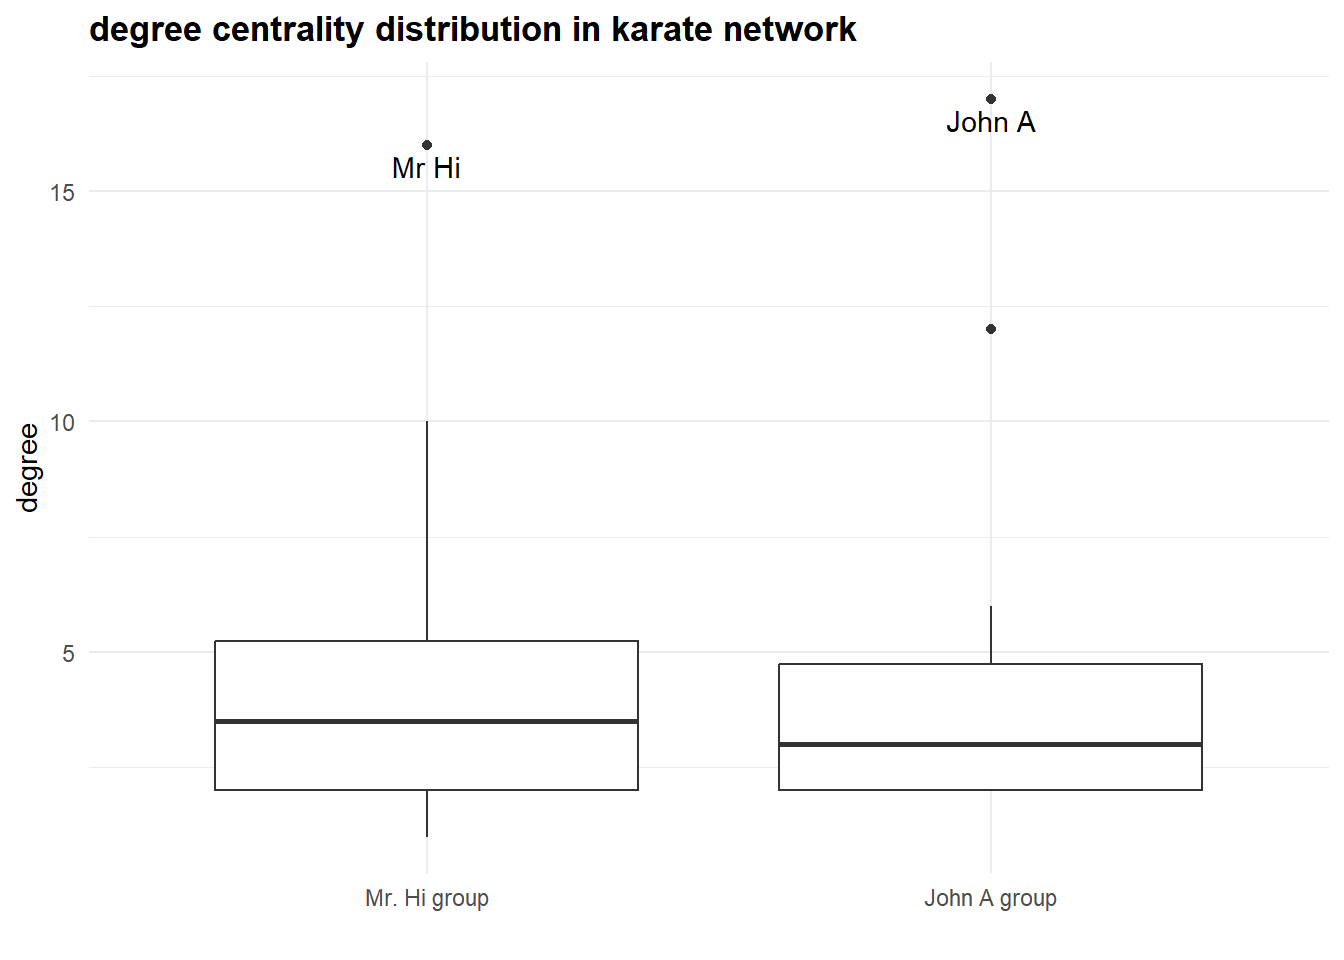
\includegraphics{chapter1_files/figure-latex/unnamed-chunk-17-1.pdf}

Given this visualization and two leading degree figures in the ``allegiance'' groups, it seems to be indeed a story about two confronting groups of actors consolidating about Mr.~Hi and John A.

The next section repeats what we've done already, and shows you how to work with different sorts of connections.

\section*{\texorpdfstring{\textbf{Working through another example}}{Working through another example}}\label{working-through-another-example}
\addcontentsline{toc}{section}{\textbf{Working through another example}}

In the most common scenario, we make some calculations on networks (calculate degrees, determine the community structure, etc.) and then get these values as a data frame suitable for the further analysis (basic statistics, distributions, regressions, and so on).

In the following code, I shortly illustrate this flow using the data from Lazega (2001). Here is the data description as given in the \texttt{manynet} package:

\begin{quote}
One-mode network dataset collected by Lazega (2001) on the relations between partners in a corporate law firm called SG\&R in New England 1988-1991. This particular subset includes the 36 partners among the 71 attorneys of this firm. Nodal attributes include seniority, formal status, office in which they work, gender, lawschool they attended, their age, and how many years they had been at the firm.
\end{quote}

First, let's load the data (\texttt{ison\_lawfirm} is a function from \texttt{manynet} package which loads the data we are interested in):

\begin{Shaded}
\begin{Highlighting}[]
\DocumentationTok{\#\# load:}
\NormalTok{lawfirm }\OtherTok{\textless{}{-}}\NormalTok{ ison\_lawfirm}

\DocumentationTok{\#\# look what is inside:}
\NormalTok{lawfirm }\SpecialCharTok{\%\textgreater{}\%} 
  \CommentTok{\#as\_igraph() \%\textgreater{}\% }
  \FunctionTok{str}\NormalTok{()}
\CommentTok{\#\textgreater{} Classes \textquotesingle{}mnet\textquotesingle{}, \textquotesingle{}tbl\_graph\textquotesingle{}, \textquotesingle{}igraph\textquotesingle{}  hidden list of 10}
\CommentTok{\#\textgreater{}  $ : num 71}
\CommentTok{\#\textgreater{}  $ : logi TRUE}
\CommentTok{\#\textgreater{}  $ : num [1:2571] 0 0 0 0 0 0 0 0 0 0 ...}
\CommentTok{\#\textgreater{}  $ : num [1:2571] 1 1 3 7 16 16 16 19 38 39 ...}
\CommentTok{\#\textgreater{}  $ : NULL}
\CommentTok{\#\textgreater{}  $ : NULL}
\CommentTok{\#\textgreater{}  $ : NULL}
\CommentTok{\#\textgreater{}  $ : NULL}
\CommentTok{\#\textgreater{}  $ :List of 4}
\CommentTok{\#\textgreater{}   ..$ : num [1:3] 1 0 1}
\CommentTok{\#\textgreater{}   ..$ :List of 3}
\CommentTok{\#\textgreater{}   .. ..$ name : chr "Lazega\textquotesingle{}s Lawyers"}
\CommentTok{\#\textgreater{}   .. ..$ grand: NULL}
\CommentTok{\#\textgreater{}   .. ..$ nodes: chr "attorneys"}
\CommentTok{\#\textgreater{}   ..$ :List of 7}
\CommentTok{\#\textgreater{}   .. ..$ status   : chr [1:71] "partner" "partner" "partner" "partner" ...}
\CommentTok{\#\textgreater{}   .. ..$ gender   : chr [1:71] "man" "man" "man" "man" ...}
\CommentTok{\#\textgreater{}   .. ..$ office   : chr [1:71] "Boston" "Boston" "Hartford" "Boston" ...}
\CommentTok{\#\textgreater{}   .. ..$ seniority: num [1:71] 31 32 13 31 31 29 29 28 25 25 ...}
\CommentTok{\#\textgreater{}   .. ..$ age      : num [1:71] 64 62 67 59 59 55 63 53 53 53 ...}
\CommentTok{\#\textgreater{}   .. ..$ practice : chr [1:71] "litigation" "corporate" "litigation" "corporate" ...}
\CommentTok{\#\textgreater{}   .. ..$ school   : chr [1:71] "Harvard/Yale" "Harvard/Yale" "Harvard/Yale" "Other" ...}
\CommentTok{\#\textgreater{}   ..$ :List of 1}
\CommentTok{\#\textgreater{}   .. ..$ type: chr [1:2571] "friends" "advice" "friends" "friends" ...}
\CommentTok{\#\textgreater{}  $ :\textless{}environment: 0x000001b54d0b5008\textgreater{} }
\CommentTok{\#\textgreater{}  {-} attr(*, "active")= chr "nodes"}
\end{Highlighting}
\end{Shaded}

As you can see, the laoded object is already a network. Note how the data is structured:

\begin{enumerate}
\def\labelenumi{(\arabic{enumi})}
\item
  in total, there are 71 nodes and 2571 edges. It should be noted that the network as it is now combines multiple types of ties (during the class we discussed that it is not a good idea), though we should be careful with interpreting the output like this.
\item
  vertex attributes (there are many of them),
\item
  edges are also differentiated (this is the only edge attribute; it is the only ``attr'' containing ``(e/c)'' caption),
\item
  the ties are directed and unweighted, - so, people in the network might have chosen each other asymetrically, but all the ties were treated equally.
\end{enumerate}

Below, we dissolve this network into nodelist and edgelist just to recreate the graph again. This procedure is for the learning purposes only: I want to remind you how (1) to get nodelist/edgelist from the ``igraph'' object and (2) to create it using these same types of data.

\begin{Shaded}
\begin{Highlighting}[]
\DocumentationTok{\#\# if you do not remember the output of the \textasciigrave{}asDF()\textasciigrave{} function}
\DocumentationTok{\#\# or struggle to understand the code below, run:}

\DocumentationTok{\#\# ison\_lawfirm \%\textgreater{}\%}
\DocumentationTok{\#\#  asDF()}

\DocumentationTok{\#\# it brings you}
\DocumentationTok{\#\#  (1) edgelist and}
\DocumentationTok{\#\#  (2) vertex list; below we refer to them immideately after the convertion:}

\DocumentationTok{\#\# nodelist:}
\NormalTok{nodelist }\OtherTok{\textless{}{-}}\NormalTok{ (lawfirm }\SpecialCharTok{\%\textgreater{}\%} 
  \FunctionTok{asDF}\NormalTok{())}\SpecialCharTok{$}\NormalTok{vertexes}

\DocumentationTok{\#\# edgelist:}
\NormalTok{edgelist }\OtherTok{\textless{}{-}}\NormalTok{ (lawfirm }\SpecialCharTok{\%\textgreater{}\%} 
  \FunctionTok{asDF}\NormalTok{())}\SpecialCharTok{$}\NormalTok{edge}

\DocumentationTok{\#\# remember about the alternative igraph functions to create the graph.}
\DocumentationTok{\#\# Here are some of them:}

\CommentTok{\# graph\_from\_adj\_list()}
\CommentTok{\# graph\_from\_edgelist()}
\CommentTok{\# graph\_from\_adjacency\_matrix()}

\NormalTok{lawfirm2 }\OtherTok{\textless{}{-}} \FunctionTok{graph\_from\_data\_frame}\NormalTok{(}
\NormalTok{  edgelist, }\DocumentationTok{\#\# (first 2 columns are taken as "edges")}
  \AttributeTok{vertices =}\NormalTok{ nodelist, }\DocumentationTok{\#\# (first column taken as id)}
  \AttributeTok{directed =}\NormalTok{ T }\DocumentationTok{\#\# it is directed by default, though.}
               \DocumentationTok{\#\# we need to specify this argument (differently)}
               \DocumentationTok{\#\# when we work with undirected networks}
\NormalTok{  )}

\NormalTok{lawfirm2}
\CommentTok{\#\textgreater{} IGRAPH d68ce7e DN{-}{-} 71 2571 {-}{-} }
\CommentTok{\#\textgreater{} + attr: name (v/c), status (v/c), gender (v/c),}
\CommentTok{\#\textgreater{} | office (v/c), seniority (v/n), age (v/n), practice}
\CommentTok{\#\textgreater{} | (v/c), school (v/c), type (e/c)}
\CommentTok{\#\textgreater{} + edges from d68ce7e (vertex names):}
\CommentTok{\#\textgreater{}  [1] 1{-}\textgreater{}2  1{-}\textgreater{}2  1{-}\textgreater{}4  1{-}\textgreater{}8  1{-}\textgreater{}17 1{-}\textgreater{}17 1{-}\textgreater{}17 1{-}\textgreater{}20 1{-}\textgreater{}39}
\CommentTok{\#\textgreater{} [10] 1{-}\textgreater{}40 1{-}\textgreater{}41 1{-}\textgreater{}56 1{-}\textgreater{}57 2{-}\textgreater{}1  2{-}\textgreater{}6  2{-}\textgreater{}7  2{-}\textgreater{}10 2{-}\textgreater{}16}
\CommentTok{\#\textgreater{} [19] 2{-}\textgreater{}16 2{-}\textgreater{}17 2{-}\textgreater{}17 2{-}\textgreater{}17 2{-}\textgreater{}20 2{-}\textgreater{}22 2{-}\textgreater{}22 2{-}\textgreater{}22 2{-}\textgreater{}24}
\CommentTok{\#\textgreater{} [28] 2{-}\textgreater{}26 2{-}\textgreater{}26 2{-}\textgreater{}26 2{-}\textgreater{}29 2{-}\textgreater{}34 2{-}\textgreater{}44 2{-}\textgreater{}45 2{-}\textgreater{}53 2{-}\textgreater{}62}
\CommentTok{\#\textgreater{} [37] 2{-}\textgreater{}64 3{-}\textgreater{}2  3{-}\textgreater{}6  3{-}\textgreater{}14 3{-}\textgreater{}14 3{-}\textgreater{}17 3{-}\textgreater{}18 3{-}\textgreater{}18 3{-}\textgreater{}25}
\CommentTok{\#\textgreater{} [46] 3{-}\textgreater{}28 3{-}\textgreater{}28 3{-}\textgreater{}30 3{-}\textgreater{}30 3{-}\textgreater{}35 4{-}\textgreater{}1  4{-}\textgreater{}2  4{-}\textgreater{}2  4{-}\textgreater{}3 }
\CommentTok{\#\textgreater{} + ... omitted several edges}
\end{Highlighting}
\end{Shaded}

Let's now split the existing network into multiple networks with the respective types of ties. First, here are these types (we can take a look at them, as we already have the edgelist):

\begin{Shaded}
\begin{Highlighting}[]
\NormalTok{edgelist }\SpecialCharTok{\%\textgreater{}\%} 
  \FunctionTok{count}\NormalTok{(type)}
\CommentTok{\#\textgreater{}      type    n}
\CommentTok{\#\textgreater{} 1  advice  892}
\CommentTok{\#\textgreater{} 2  cowork 1104}
\CommentTok{\#\textgreater{} 3 friends  575}
\end{Highlighting}
\end{Shaded}

This result is already telling: there are twice more coworking ties among the studied colleagues than friendship ties. Next, we can create separate networks for each type of ties:

\begin{Shaded}
\begin{Highlighting}[]
\DocumentationTok{\#\# advice network:}
\NormalTok{g.advice }\OtherTok{\textless{}{-}}\NormalTok{ edgelist }\SpecialCharTok{\%\textgreater{}\%} 
  \FunctionTok{filter}\NormalTok{(type }\SpecialCharTok{==} \StringTok{"advice"}\NormalTok{) }\SpecialCharTok{\%\textgreater{}\%}
  
  \DocumentationTok{\#\# we can also write these lines as a first argument inside}
  \DocumentationTok{\#\# \textasciigrave{}graph\_from\_data\_frame()\textasciigrave{}}
  
  \FunctionTok{graph\_from\_data\_frame}\NormalTok{(}\AttributeTok{vertices =}\NormalTok{ nodelist,}
                        \AttributeTok{directed =}\NormalTok{ T)}

\DocumentationTok{\#\# cowork network:}
\NormalTok{g.cowork }\OtherTok{\textless{}{-}}\NormalTok{ edgelist }\SpecialCharTok{\%\textgreater{}\%} 
  \FunctionTok{filter}\NormalTok{(type }\SpecialCharTok{==} \StringTok{"cowork"}\NormalTok{) }\SpecialCharTok{\%\textgreater{}\%}
  \FunctionTok{graph\_from\_data\_frame}\NormalTok{(}\AttributeTok{vertices =}\NormalTok{ nodelist,}
                        \AttributeTok{directed =}\NormalTok{ T)}

\DocumentationTok{\#\# friendship network:}
\NormalTok{g.friends }\OtherTok{\textless{}{-}}\NormalTok{ edgelist }\SpecialCharTok{\%\textgreater{}\%} 
  \FunctionTok{filter}\NormalTok{(type }\SpecialCharTok{==} \StringTok{"friends"}\NormalTok{) }\SpecialCharTok{\%\textgreater{}\%}
  \FunctionTok{graph\_from\_data\_frame}\NormalTok{(}\AttributeTok{vertices =}\NormalTok{ nodelist,}
                        \AttributeTok{directed =}\NormalTok{ T)}
\end{Highlighting}
\end{Shaded}

Note the naming for the ``igraph'' objects: it usually (in tutorials from online, for example) use ``g'' for graphs = networks. In our case, we also differentiate using the ties used in them.

Now it is legitimate to build these networks - once again, we do not want to mix the ties in our analysis to be sure about the real micro-/macro- consequences of the particular types of ties. So, let's look at these networks.

One fancy procedure is done here that we did not cover yet - to plot the networks, I calculate the network centralities for all the nodes in each network. Degree centrality is the number of ties a node has; in the context of directred networks it might specifically calculate incoming our outgoing ties. Here, we calculate the incoming degree centrality, i.e.~the number of ties a node receive.

Also, to make the pictures more interesting and remind you the way to use node attributes, I color the nodes using the \texttt{office} variable from the nodelist.

\begin{Shaded}
\begin{Highlighting}[]
\DocumentationTok{\#\# degree centralities calculation:}
\FunctionTok{V}\NormalTok{(g.advice)}\SpecialCharTok{$}\NormalTok{degree }\OtherTok{=} \FunctionTok{degree}\NormalTok{(g.advice, }\AttributeTok{mode =} \StringTok{"in"}\NormalTok{)}
\FunctionTok{V}\NormalTok{(g.cowork)}\SpecialCharTok{$}\NormalTok{degree }\OtherTok{=} \FunctionTok{degree}\NormalTok{(g.cowork, }\AttributeTok{mode =} \StringTok{"in"}\NormalTok{)}
\FunctionTok{V}\NormalTok{(g.friends)}\SpecialCharTok{$}\NormalTok{degree }\OtherTok{=} \FunctionTok{degree}\NormalTok{(g.friends, }\AttributeTok{mode =} \StringTok{"in"}\NormalTok{)}

\FunctionTok{set.seed}\NormalTok{(}\DecValTok{42}\NormalTok{)}
\DocumentationTok{\#\# below is a large code which:}
\CommentTok{\# 1. makes 3 networks}
\CommentTok{\# 2. ties them together}
\DocumentationTok{\#\# feel free to tear it apart to figure out what happens}
\DocumentationTok{\#\# (change values, colors, variables, etc.)}
\DocumentationTok{\#\# {-}{-}\textgreater{} that is a great way to learn network analysis!}

\CommentTok{\# (the comments regarding the plotting are given for the first network)}

\FunctionTok{par}\NormalTok{(}\AttributeTok{mfrow =} \FunctionTok{c}\NormalTok{(}\DecValTok{1}\NormalTok{,}\DecValTok{3}\NormalTok{))}

\DocumentationTok{\#\# advice network:}
\FunctionTok{par}\NormalTok{(}\AttributeTok{mar=}\FunctionTok{c}\NormalTok{(}\DecValTok{0}\NormalTok{,}\DecValTok{0}\NormalTok{,}\DecValTok{0}\NormalTok{,}\DecValTok{0}\NormalTok{)) }\DocumentationTok{\#\# better to include when plotting, increase image size}
\NormalTok{g.advice }\SpecialCharTok{\%\textgreater{}\%} 
  \FunctionTok{plot}\NormalTok{(}\AttributeTok{vertex.label =} \ConstantTok{NA}\NormalTok{, }\DocumentationTok{\#\# labels are almost always messy}
       
       \DocumentationTok{\#\# one of the ways to match values to colors;}
       \DocumentationTok{\#\# otherwise, assign colors to a nodelist column and use it directly}
       \AttributeTok{vertex.color =} \FunctionTok{ifelse}\NormalTok{(}\FunctionTok{V}\NormalTok{(g.advice)}\SpecialCharTok{$}\NormalTok{office }\SpecialCharTok{==} \StringTok{"Boston"}\NormalTok{, }
                             \StringTok{"lightblue"}\NormalTok{,}
                             \FunctionTok{ifelse}\NormalTok{(}\FunctionTok{V}\NormalTok{(g.advice)}\SpecialCharTok{$}\NormalTok{office }\SpecialCharTok{==} \StringTok{"Hartford"}\NormalTok{,}
                             \StringTok{"coral1"}\NormalTok{,}
                             \StringTok{"lightgreen"}\NormalTok{)),}
       
       \DocumentationTok{\#\# use degree calculated earlier + decrease sizes using division by 2}
       \AttributeTok{vertex.size =} \FunctionTok{V}\NormalTok{(g.advice)}\SpecialCharTok{$}\NormalTok{degree }\SpecialCharTok{/} \DecValTok{2}\NormalTok{,}
       
       \AttributeTok{edge.color =} \StringTok{"grey70"}\NormalTok{, }\DocumentationTok{\#\# just the color for edges}
       \AttributeTok{edge.arrow.width =} \FloatTok{0.2}\NormalTok{, }\DocumentationTok{\#\# size of the arrow}
       
       \DocumentationTok{\#\# igraph is sensitive to new lines {-} by using it,}
       \DocumentationTok{\#\# we can arrange the titles for graphs nicely}
       \DocumentationTok{\#\# (and include some descriptions there as well)}
       \AttributeTok{main =} \StringTok{"}\SpecialCharTok{\textbackslash{}n\textbackslash{}n\textbackslash{}n}\StringTok{advice}\SpecialCharTok{\textbackslash{}n}\StringTok{(892 ties)"}\NormalTok{)}

\DocumentationTok{\#\# cowork network:}
\FunctionTok{par}\NormalTok{(}\AttributeTok{mar=}\FunctionTok{c}\NormalTok{(}\DecValTok{0}\NormalTok{,}\DecValTok{0}\NormalTok{,}\DecValTok{0}\NormalTok{,}\DecValTok{0}\NormalTok{))}
\NormalTok{g.cowork }\SpecialCharTok{\%\textgreater{}\%} 
  \FunctionTok{plot}\NormalTok{(}\AttributeTok{vertex.label =} \ConstantTok{NA}\NormalTok{,}
       \AttributeTok{vertex.color =} \FunctionTok{ifelse}\NormalTok{(}\FunctionTok{V}\NormalTok{(g.cowork)}\SpecialCharTok{$}\NormalTok{office }\SpecialCharTok{==} \StringTok{"Boston"}\NormalTok{,}
                             \StringTok{"lightblue"}\NormalTok{,}
                             \FunctionTok{ifelse}\NormalTok{(}\FunctionTok{V}\NormalTok{(g.cowork)}\SpecialCharTok{$}\NormalTok{office }\SpecialCharTok{==} \StringTok{"Hartford"}\NormalTok{,}
                             \StringTok{"coral1"}\NormalTok{,}
                             \StringTok{"lightgreen"}\NormalTok{)),}
       \AttributeTok{vertex.size =} \FunctionTok{V}\NormalTok{(g.cowork)}\SpecialCharTok{$}\NormalTok{degree }\SpecialCharTok{/} \DecValTok{2}\NormalTok{,}
       \AttributeTok{edge.width =} \FunctionTok{seq}\NormalTok{(}\FloatTok{0.5}\NormalTok{, }\FloatTok{0.08}\NormalTok{),}
       \AttributeTok{edge.color =} \StringTok{"grey70"}\NormalTok{,}
       \AttributeTok{edge.arrow.width =} \FloatTok{0.2}\NormalTok{,}
       \AttributeTok{main =} \StringTok{"}\SpecialCharTok{\textbackslash{}n\textbackslash{}n\textbackslash{}n}\StringTok{cowork}\SpecialCharTok{\textbackslash{}n}\StringTok{(1104 ties)"}\NormalTok{)}

\DocumentationTok{\#\# friends network:}
\FunctionTok{par}\NormalTok{(}\AttributeTok{mar=}\FunctionTok{c}\NormalTok{(}\DecValTok{0}\NormalTok{,}\DecValTok{0}\NormalTok{,}\DecValTok{0}\NormalTok{,}\DecValTok{0}\NormalTok{))}
\NormalTok{g.friends }\SpecialCharTok{\%\textgreater{}\%} 
  \FunctionTok{plot}\NormalTok{(}\AttributeTok{vertex.label =} \ConstantTok{NA}\NormalTok{,}
       \AttributeTok{vertex.color =} \FunctionTok{ifelse}\NormalTok{(}\FunctionTok{V}\NormalTok{(g.friends)}\SpecialCharTok{$}\NormalTok{office }\SpecialCharTok{==} \StringTok{"Boston"}\NormalTok{,}
                             \StringTok{"lightblue"}\NormalTok{,}
                             \FunctionTok{ifelse}\NormalTok{(}\FunctionTok{V}\NormalTok{(g.friends)}\SpecialCharTok{$}\NormalTok{office }\SpecialCharTok{==} \StringTok{"Hartford"}\NormalTok{,}
                             \StringTok{"coral1"}\NormalTok{,}
                             \StringTok{"lightgreen"}\NormalTok{)),}
       \AttributeTok{vertex.size =} \FunctionTok{V}\NormalTok{(g.friends)}\SpecialCharTok{$}\NormalTok{degree,}
       \AttributeTok{edge.width =} \FunctionTok{seq}\NormalTok{(}\FloatTok{0.5}\NormalTok{, }\FloatTok{0.08}\NormalTok{),}
       \AttributeTok{edge.color =} \StringTok{"grey70"}\NormalTok{,}
       \AttributeTok{edge.arrow.width =} \FloatTok{0.2}\NormalTok{,}
       \AttributeTok{main =} \StringTok{"}\SpecialCharTok{\textbackslash{}n\textbackslash{}n\textbackslash{}n}\StringTok{friends}\SpecialCharTok{\textbackslash{}n}\StringTok{(575 ties)"}\NormalTok{)}

\FunctionTok{legend}\NormalTok{(}
  \StringTok{"bottomright"}\NormalTok{,}
  \AttributeTok{pch =} \DecValTok{21}\NormalTok{,}
  \AttributeTok{legend =} \FunctionTok{c}\NormalTok{(}\StringTok{"Boston"}\NormalTok{, }\StringTok{"Hartford"}\NormalTok{, }\StringTok{"Providence"}\NormalTok{),}
  \AttributeTok{pt.cex =} \FloatTok{1.5}\NormalTok{,}
  \AttributeTok{pt.bg =} \FunctionTok{c}\NormalTok{(}\StringTok{"lightblue"}\NormalTok{, }\StringTok{"coral1"}\NormalTok{, }\StringTok{"palegreen3"}\NormalTok{),}
  \AttributeTok{col =} \StringTok{"black"}\NormalTok{,}
  \AttributeTok{bty =} \StringTok{"n"}\NormalTok{)}
\end{Highlighting}
\end{Shaded}

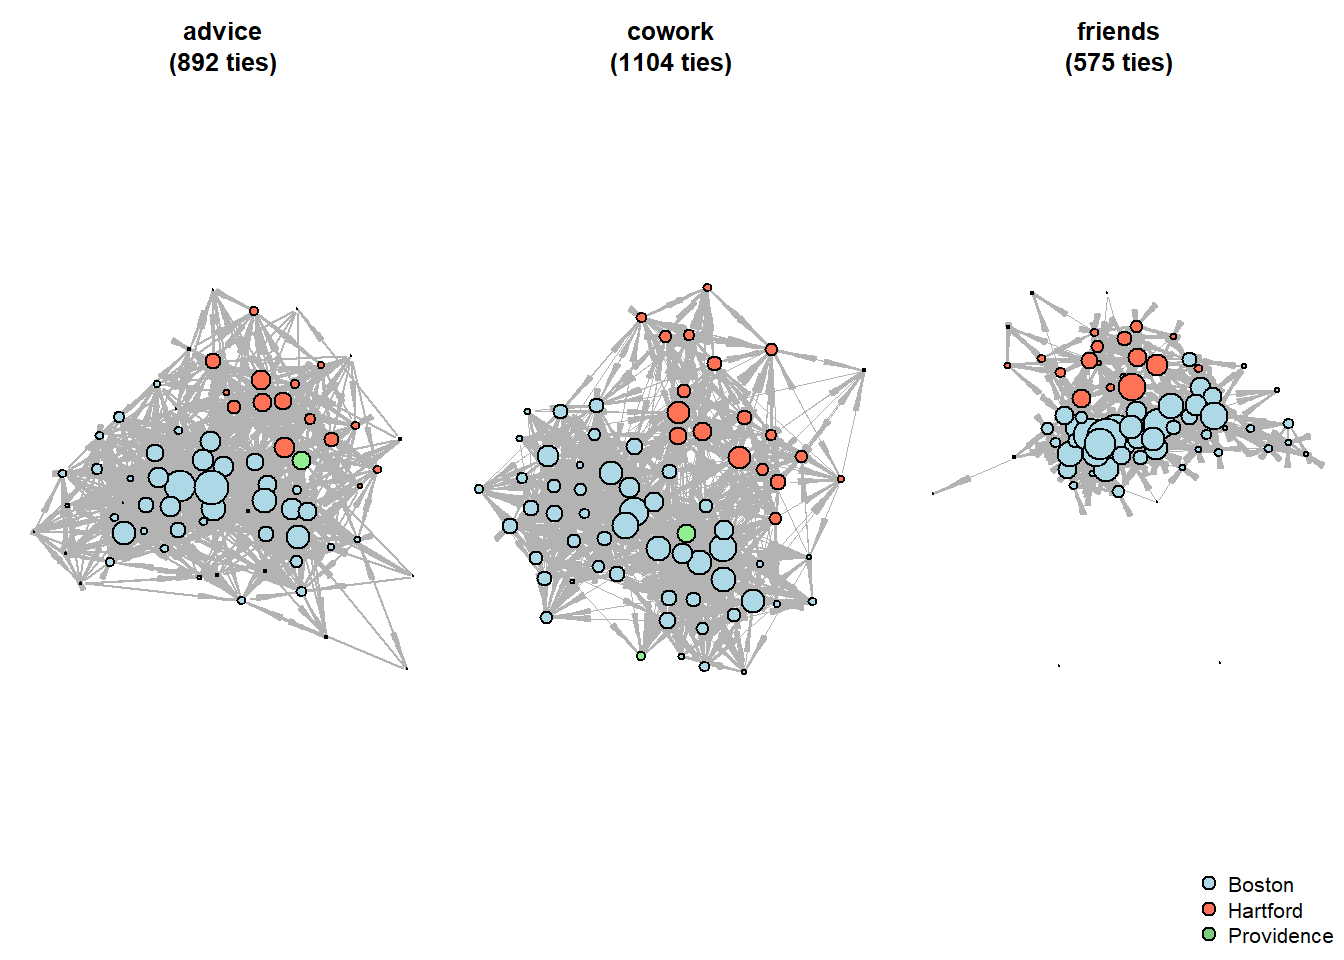
\includegraphics{chapter1_files/figure-latex/unnamed-chunk-22-1.pdf}

Although the pictures are useful \& engaging, some articles on networks do not include them at all. In our case, they provide little insight to the actual differences among the networks. To finish this set of analysis, we will just return to the nodelists once again and compare the average numbers of degrees across the offices (mean highest degree centralities).

\begin{Shaded}
\begin{Highlighting}[]
\NormalTok{(g.advice }\SpecialCharTok{\%\textgreater{}\%} 
  \FunctionTok{asDF}\NormalTok{())}\SpecialCharTok{$}\NormalTok{vertex }\SpecialCharTok{\%\textgreater{}\%} \DocumentationTok{\#\# get nodelist}
  \FunctionTok{select}\NormalTok{(intergraph\_id, office, degree) }\SpecialCharTok{\%\textgreater{}\%} 
  \DocumentationTok{\#\# (we need intergraph\_id to further join with other nodelists)}
  \FunctionTok{rename}\NormalTok{(}\AttributeTok{degree\_advice =}\NormalTok{ degree) }\SpecialCharTok{\%\textgreater{}\%} 
  
  \FunctionTok{left\_join}\NormalTok{((g.cowork }\SpecialCharTok{\%\textgreater{}\%}
               \FunctionTok{asDF}\NormalTok{())}\SpecialCharTok{$}\NormalTok{vertex }\SpecialCharTok{\%\textgreater{}\%}
              \FunctionTok{select}\NormalTok{(intergraph\_id, office, degree) }\SpecialCharTok{\%\textgreater{}\%}
              \FunctionTok{rename}\NormalTok{(}\AttributeTok{degree\_cowork =}\NormalTok{ degree)) }\SpecialCharTok{\%\textgreater{}\%} 
    
    \FunctionTok{left\_join}\NormalTok{((g.friends }\SpecialCharTok{\%\textgreater{}\%}
                 \FunctionTok{asDF}\NormalTok{())}\SpecialCharTok{$}\NormalTok{vertex }\SpecialCharTok{\%\textgreater{}\%}
                \FunctionTok{select}\NormalTok{(intergraph\_id, office, degree) }\SpecialCharTok{\%\textgreater{}\%}
                \FunctionTok{rename}\NormalTok{(}\AttributeTok{degree\_friends =}\NormalTok{ degree)) }\SpecialCharTok{\%\textgreater{}\%} 
  
  \FunctionTok{group\_by}\NormalTok{(office) }\SpecialCharTok{\%\textgreater{}\%} 
  \FunctionTok{summarise}\NormalTok{(}\AttributeTok{n\_employees =} \FunctionTok{n}\NormalTok{(),}
            \AttributeTok{average\_advice =} \FunctionTok{round}\NormalTok{(}\FunctionTok{mean}\NormalTok{(degree\_advice),}\DecValTok{2}\NormalTok{),}
            \AttributeTok{average\_cowork =} \FunctionTok{round}\NormalTok{(}\FunctionTok{mean}\NormalTok{(degree\_cowork),}\DecValTok{2}\NormalTok{),}
            \AttributeTok{average\_friends =} \FunctionTok{round}\NormalTok{(}\FunctionTok{mean}\NormalTok{(degree\_friends),}\DecValTok{2}\NormalTok{))}
\CommentTok{\#\textgreater{} Joining with \textasciigrave{}by = join\_by(intergraph\_id, office)\textasciigrave{}}
\CommentTok{\#\textgreater{} Joining with \textasciigrave{}by = join\_by(intergraph\_id, office)\textasciigrave{}}
\CommentTok{\#\textgreater{} \# A tibble: 3 x 5}
\CommentTok{\#\textgreater{}   office     n\_employees average\_advice average\_cowork}
\CommentTok{\#\textgreater{}   \textless{}chr\textgreater{}            \textless{}int\textgreater{}          \textless{}dbl\textgreater{}          \textless{}dbl\textgreater{}}
\CommentTok{\#\textgreater{} 1 Boston              48          13.6            16.5}
\CommentTok{\#\textgreater{} 2 Hartford            19          11.3            14.4}
\CommentTok{\#\textgreater{} 3 Providence           4           6.25           10.2}
\CommentTok{\#\textgreater{} \# i 1 more variable: average\_friends \textless{}dbl\textgreater{}}
\end{Highlighting}
\end{Shaded}

It is hard to interpret the table straightforwardly as far as the different numbers of people are involved in each office. Still, we see that the average degree values are higher for Boston than Hartford, and Providence employees are excluded from the friendship network almost entirely. Sad but not that surprising given their office size.

Likewise, we can calculate the more specific stories, like the average number of people who ask women employees for advice. It is interesting that females are not discriminated (in this pure basic mathematical metrics) in friendship network:

\begin{Shaded}
\begin{Highlighting}[]
\NormalTok{(g.advice }\SpecialCharTok{\%\textgreater{}\%} 
  \FunctionTok{asDF}\NormalTok{())}\SpecialCharTok{$}\NormalTok{vertex }\SpecialCharTok{\%\textgreater{}\%} 
  \FunctionTok{group\_by}\NormalTok{(gender) }\SpecialCharTok{\%\textgreater{}\%} 
  \FunctionTok{summarise}\NormalTok{(}\AttributeTok{n\_employees =} \FunctionTok{n}\NormalTok{(),}
            \AttributeTok{mean\_advice =} \FunctionTok{round}\NormalTok{(}\FunctionTok{mean}\NormalTok{(degree),}\DecValTok{2}\NormalTok{)) }\SpecialCharTok{\%\textgreater{}\%} 
  
  \FunctionTok{left\_join}\NormalTok{((g.friends }\SpecialCharTok{\%\textgreater{}\%}
               \FunctionTok{asDF}\NormalTok{())}\SpecialCharTok{$}\NormalTok{vertex }\SpecialCharTok{\%\textgreater{}\%}
              \FunctionTok{group\_by}\NormalTok{(gender) }\SpecialCharTok{\%\textgreater{}\%}
              \FunctionTok{summarise}\NormalTok{(}\AttributeTok{mean\_friends =} \FunctionTok{round}\NormalTok{(}\FunctionTok{mean}\NormalTok{(degree),}\DecValTok{2}\NormalTok{)))}
\CommentTok{\#\textgreater{} Joining with \textasciigrave{}by = join\_by(gender)\textasciigrave{}}
\CommentTok{\#\textgreater{} \# A tibble: 2 x 4}
\CommentTok{\#\textgreater{}   gender n\_employees mean\_advice mean\_friends}
\CommentTok{\#\textgreater{}   \textless{}chr\textgreater{}        \textless{}int\textgreater{}       \textless{}dbl\textgreater{}        \textless{}dbl\textgreater{}}
\CommentTok{\#\textgreater{} 1 man             53       14.0          8.06}
\CommentTok{\#\textgreater{} 2 woman           18        8.28         8.22}
\end{Highlighting}
\end{Shaded}

As a final example, we can plot seniority (years of experience in a company) against the number of advices an employee provided:

\begin{Shaded}
\begin{Highlighting}[]
\NormalTok{(g.advice }\SpecialCharTok{\%\textgreater{}\%} 
  \FunctionTok{asDF}\NormalTok{())}\SpecialCharTok{$}\NormalTok{vertex }\SpecialCharTok{\%\textgreater{}\%} 
  
  \FunctionTok{ggplot}\NormalTok{(}\FunctionTok{aes}\NormalTok{(seniority, degree)) }\SpecialCharTok{+}
  \FunctionTok{geom\_point}\NormalTok{() }\SpecialCharTok{+}
  \FunctionTok{geom\_smooth}\NormalTok{() }\SpecialCharTok{+}
  \FunctionTok{labs}\NormalTok{(}\AttributeTok{y =} \StringTok{"in{-}degree in advice network}\SpecialCharTok{\textbackslash{}n}\StringTok{"}\NormalTok{,}
       \AttributeTok{subtitle =} \StringTok{"The effect of seniority on centrality }
\StringTok{       in advice network }\SpecialCharTok{\textbackslash{}n}\StringTok{is diminished after 10+ years of work"}\NormalTok{) }\SpecialCharTok{+}
  \FunctionTok{theme\_minimal}\NormalTok{() }\SpecialCharTok{+}
  \FunctionTok{theme}\NormalTok{(}\AttributeTok{plot.subtitle =} \FunctionTok{element\_text}\NormalTok{(}\AttributeTok{face=}\StringTok{\textquotesingle{}bold\textquotesingle{}}\NormalTok{))}
\end{Highlighting}
\end{Shaded}

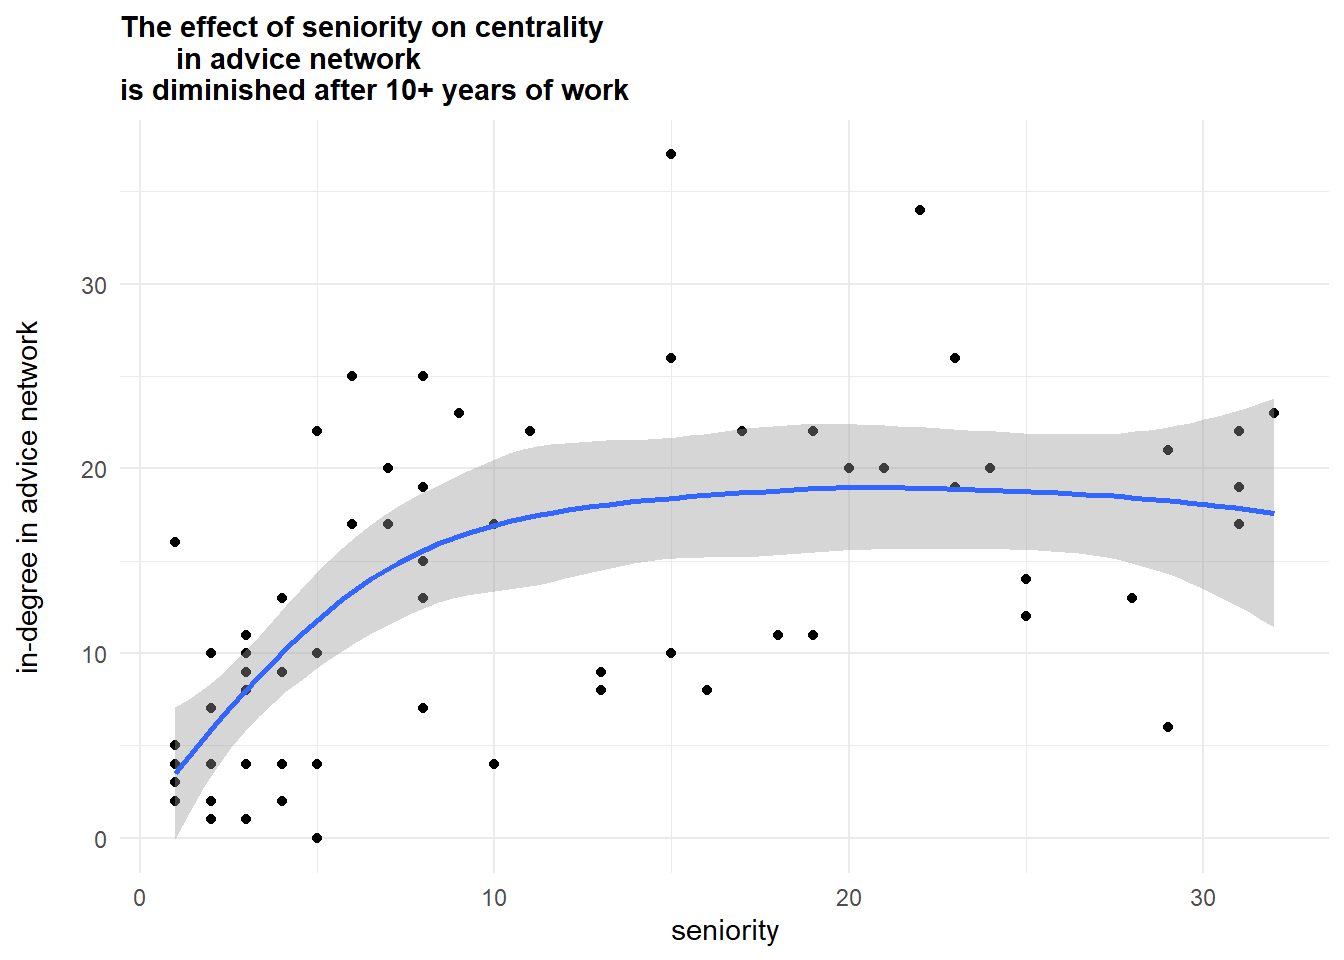
\includegraphics{chapter1_files/figure-latex/unnamed-chunk-25-1.pdf}

\section*{\texorpdfstring{\textbf{Conclusion}}{Conclusion}}\label{conclusion}
\addcontentsline{toc}{section}{\textbf{Conclusion}}

You are now familiar with a basic network analysis routine as it looks in R. Keep in mind (1) data formats: matrices and edgelists/nodelists, as well as conversions from one format to another, and (2) the possibilities of ``regular'' descriptive/statistical work with the indicators derived from your networks.

Articles mentioned in the text:

\begin{itemize}
\item
  Lazega, E. (2001). The collegial phenomenon: The social mechanisms of cooperation among peers in a corporate law partnership. Oxford University Press, USA.
\item
  Zachary, W. W. (1977). An information flow model for conflict and fission in small groups. Journal of anthropological research, 33(4), 452-473.
\end{itemize}

\chapter*{\texorpdfstring{\textbf{Chapter 2}}{Chapter 2}}\label{chapter-2}
\addcontentsline{toc}{chapter}{\textbf{Chapter 2}}

\begin{quote}
\emph{work-in-progress }
\end{quote}

\chapter*{\texorpdfstring{(PART*) \textbf{Appendices}}{(PART*) Appendices}}\label{part-appendices}
\addcontentsline{toc}{chapter}{(PART*) \textbf{Appendices}}

\chapter*{\texorpdfstring{\textbf{Available datasets}}{Available datasets}}\label{available-datasets}
\addcontentsline{toc}{chapter}{\textbf{Available datasets}}

Throughout the course I will do my best to illustrate network-related ideas using various sources of data, e.g.~from organizational domains to pupils' interactions and from well-known and ``modal'' (typically used in tutorials) to those found in recent academic and non-academic publications and collected by me. Still, for the exam project and 3 out of 4 home assignments which involve programming, you will need to pick a dataset to work with. The list below provides some basic sources of data which you can use for your investigations:

Other highly recommended platforms include GitHub and similar data-sharing sites (see the list below). Many enthusiasts collect and upload network data there, and sometimes these authors also provide accompanying learning materials.

\begin{itemize}
\item
  R packages, like \href{https://cran.r-project.org/web/packages/manynet/manynet.pdf}{``manynet''} and, especially, \href{https://schochastics.github.io/networkdata/}{``networkdata''}, assemble many network datasets and provide easy access to them. Be aware that the ``networkdata'' package can take a while to install, as it includes nearly a thousand datasets. I recommend installing both, as I will sometimes use data from these libraries during practical sessions.
\item
  \href{https://networkdata.ics.uci.edu/index.html}{The UCI Network Data Repository} is another wonderful source, where datasets are tagged by their subject and the phenomena they represent. Please note that some files may be in atypical formats, so you might need to convert them into an R-suitable format for your work.
\item
  \href{https://sites.google.com/site/ucinetsoftware/datasets}{Datasets} provided by UCINET software developers are in Pajek format (these can be used in R with some manipulation), but you will likely find most of these networks in aforementioned ``networkdata'' package.
\item
  Other highly recommended platforms include github and similar data-sharing sites (see some more in the next list). Many enthusiasts collect and upload network data there, and sometimes these authors also provide accompanying learning materials, e.g.~\href{https://github.com/JeffreyAlanSmith/Integrated_Network_Science/tree/master/data}{here}.
\end{itemize}

Obviously, these sources do not cover the full variety of networks available. Here are some examples of datasets that previous generation of students has found on their own:

\begin{itemize}
\item
  \href{https://www.kaggle.com/datasets/andreagarritano/deezer-social-networks}{Networks of \emph{Deezer} users in three countries}, available at kaggle.com
\item
  A \href{https://dracor.org/rus}{collection} of networks based on character interactions in Russian drama literature (similar collections are also available for other languages and literatures).
\item
  \href{https://dataverse.pushdom.ru/dataset.xhtml?persistentId=doi:10.31860/openlit-2023.4-B003}{Russian-European literature connections of 18 century}, another literature-related source.
\end{itemize}

Finally, remember that you can collect data yourself. During the course, I will show you examples of not-too-large datasets collected in seconds using the web-scraping techniques.

\chapter*{\texorpdfstring{\textbf{Intro to web-scraping}}{Intro to web-scraping}}\label{intro-to-web-scraping}
\addcontentsline{toc}{chapter}{\textbf{Intro to web-scraping}}

TBA

\begin{quote}
\emph{work-in-progress: (1) see .Rmd for sixth meeting from last year, on Wiki: can change it to example on sociologists, (2) maybe introduce Selenium / parallel computing, or (3) provide more different examples}
\end{quote}

\chapter*{\texorpdfstring{\textbf{Recommended literature}}{Recommended literature}}\label{recommended-literature}
\addcontentsline{toc}{chapter}{\textbf{Recommended literature}}

\begin{quote}
\emph{work-in-progress: (1) literature will be re-arranged more logically, (2) literature will be added, (3) maybe network viz of citation relations between these sources (?). }
\end{quote}

Although we have too little time to dive into the literature, you might want (or need) to consult some of the sources from below during the module. First, here are the technical guides which cover the basic concepts:

\begin{itemize}
\item
  Rawlings, C. M., Smith, J. A., Moody, J., \& McFarland, D. A. (2023). Network analysis: integrating social network theory, method, and application with R. Cambridge University Press.
  (on-line supplementary material is available \href{https://inarwhal.github.io/NetworkAnalysisR-book/}{here})
\item
  Hanneman R. \& Riddle M. (2005) Introduction to Social Network Methods
  (on-line book, available \href{https://faculty.ucr.edu/~hanneman/nettext/index.html}{here})
\item
  Wasserman, S. \& Faust K. (1994) Social network analysis: Methods and applications. The Press Syndicate of the University of Cambridge.
\end{itemize}

Additionally, the following list is a mixture of theoretical writings and empirical papers primarily from the field of sociology. It is also with some incline towards the sociology of science, as (1) the data on scientific activities is easily available for researchers and (2) I am interested in this subfield personally. When selecting from this list, consider both (1) the domain of inquiry (topics) that interests you and (2) the methods applied. The most exciting works (in my opinion) are marked in \textbf{bold}.

Social network analysis is widely used in other social sciences. If you need recommendations on literature for your specific interests, feel free to reach out to me during class or via email, and I will do my best to provide you with relevant and essential papers for your research.

\section*{\texorpdfstring{\textbf{History of the field and predecessors}}{History of the field and predecessors}}\label{history-of-the-field-and-predecessors}
\addcontentsline{toc}{section}{\textbf{History of the field and predecessors}}

\begin{itemize}
\item
  Freeman, L. (2004). The development of social network analysis. A Study in the Sociology of Science, 1(687), 159--167.
\item
  Freeman, L. C. (2011). The development of social network analysis--with an emphasis on recent events. The Sage handbook of social network analysis, 21(3), 26-39.
\item
  Hidalgo, C. A. (2016). Disconnected, fragmented, or united? A trans-disciplinary review of network science. Applied Network Science, 1(1), 6.
\item
  Korom, P. (2015). Network analysis, history of. In International encyclopedia of the social \& behavioral sciences (pp.~524-531). Elsevier.
\item
  Simmel, G. (2010). Conflict and the web of group affiliations. Simon and Schuster.
\item
  Wolff, K. H. (1950). The sociology of Georg Simmel. Glencoe, Ill: Free Press.
\item
  Chayko, M. (2015). The first web theorist? Georg Simmel and the legacy of `The web of group-affiliations.' Information, Communication \& Society, 18(12), 1419--1422.
\item
  Bott, E. (2014). Conjugal roles and social networks. In Family and Social Network (pp.~52--96). Routledge.
\item
  Moreno, J. L., Jennings, H. H., \& Stockton, R. (1943). Sociometry in the classroom. Sociometry, 6(4), 425-428.
\item
  Coleman, J., Katz, E., \& Menzel, H. (1957). The diffusion of an innovation among physicians. Sociometry, 20(4), 253--270.
\end{itemize}

\section*{\texorpdfstring{\textbf{Network theory \& super-influential papers}}{Network theory \& super-influential papers}}\label{network-theory-super-influential-papers}
\addcontentsline{toc}{section}{\textbf{Network theory \& super-influential papers}}

\begin{itemize}
\item
  \textbf{Granovetter, M. (1985). Economic Action and Social Structure: The Problem of Embeddedness. American Journal of Sociology, 91(3), 481--510.}
\item
  \textbf{Granovetter, M. S. (1973). The Strength of Weak Ties. American Journal of Sociology, 78(6), 1360--1380.}
\item
  Bottero, W., \& Crossley, N. (2011). Worlds, Fields and Networks: Becker, Bourdieu and the Structures of Social Relations. Cultural Sociology, 5(1), 99--119.
\item
  Emirbayer, M. (1997). Manifesto for a Relational Sociology. American Journal of Sociology, 103(2), 281--317.
\item
  \textbf{Erikson, E. (2013). Formalist and Relationalist Theory in Social Network Analysis. Sociological Theory, 31(3), 219--242.}
\item
  Fuhse, J. A. (2015). Theorizing social networks: The relational sociology of and around Harrison White. International Review of Sociology, 25(1), 15--44.
\item
  Ranjay Gulati, Sameer B. Srivastava, (2014),``Bringing Agency Back into Network Research: Constrained Agency and Network Action'', Research in the Sociology of Organizations, Vol. 40 pp.~73-93.
\item
  \textbf{Knox, H., Savage, M., \& Harvey, P. (2006). Social networks and the study of relations: Networks as method, metaphor and form. Economy and Society, 35(1), 113--140.}
\item
  \textbf{Omar Lizardo, Melissa Fletcher Pirkey, (2014),``How Organizational Theory can Help Network Theorizing: Linking Structure and Dynamics via Cross-Level Analogies'', Research in the Sociology of Organizations, Vol. 40 pp.~33-56.}
\item
  White, H. C. (1995). Social networks can resolve actor paradoxes in economics and in psychology. Journal of Institutional and Theoretical Economics (JITE)/Zeitschrift Für Die Gesamte Staatswissenschaft, 58--74.
\item
  Mische, A., \& White, H. (1998). Between conversation and situation: Public switching dynamics across network domains. Social Research, 695--724.
\item
  Crossley, N. (2010). Networks and Complexity: Directions for Interactionist Research? Symbolic Interaction, 33(3), 341--363.
\item
  Jones, C., Hesterly, W. S., \& Borgatti, S. P. (1997). A General Theory of Network Governance: Exchange Conditions and Social Mechanisms. The Academy of Management Review, 22(4), 911.
\item
  \textbf{Padgett, J. F., \& Ansell, C. K. (1993). Robust Action and the Rise of the Medici, 1400-1434. American Journal of Sociology, 98(6), 1259--1319.}
\end{itemize}

\section*{\texorpdfstring{\textbf{Topology}}{Topology}}\label{topology}
\addcontentsline{toc}{section}{\textbf{Topology}}

\begin{itemize}
\item
  \textbf{Cattani, G., \& Ferriani, S. (2008). A Core/Periphery Perspective on Individual Creative Performance: Social Networks and Cinematic Achievements in the Hollywood Film Industry. Organization Science, 19(6), 824--844.}
\item
  \textbf{Uzzi, B., \& Spiro, J. (2005). Collaboration and Creativity: The Small World Problem. American Journal of Sociology, 111(2), 447--504.}
\item
  Watts, D. J. (1999). Networks, Dynamics, and the Small‐World Phenomenon. American Journal of Sociology, 105(2), 493--527.
\item
  Blondel, V., Guillaume, J. L., \& Lambiotte, R. (2024). Fast unfolding of communities in large networks: 15 years later. Journal of Statistical Mechanics: Theory and Experiment, 2024(10), 10R001.
\item
  Young, R. C., \& Larson, O. F. (1965). A new approach to community structure. American Sociological Review, 30(6), 926-934.
\item
  \textbf{Guimerà, R., Uzzi, B., Spiro, J., \& Amaral, L. A. N. (2005). Team Assembly Mechanisms Determine Collaboration Network Structure and Team Performance. Science, 308(5722), 697--702.}
\end{itemize}

\section*{\texorpdfstring{\textbf{Network positions, centrality measures, and its consequences}}{Network positions, centrality measures, and its consequences}}\label{network-positions-centrality-measures-and-its-consequences}
\addcontentsline{toc}{section}{\textbf{Network positions, centrality measures, and its consequences}}

\begin{itemize}
\item
  Ahuja, G. (2000). Collaboration Networks, Structural Holes, and Innovation: A Longitudinal Study. Administrative Science Quarterly, 45(3), 425--455.
\item
  \textbf{Burt, R. S. (2004). Structural Holes and Good Ideas. American Journal of Sociology, 110(2), 349--399.}
\item
  Burt, R. S. (2005). Brokerage and closure: An introduction to social capital. Oxford university press.
\item
  Rossman, G., Esparza, N., \& Bonacich, P. (2010). I'd Like to Thank the Academy, Team Spillovers, and Network Centrality. American Sociological Review, 75(1), 31--51.
\item
  David Obstfeld, Stephen P. Borgatti, Jason Davis, (2014),``Brokerage as a Process: Decoupling Third Party Action from Social Network Structure'', Research in the Sociology of Organizations, Vol. 40 pp.~135-159
\end{itemize}

\section*{\texorpdfstring{\textbf{Two-mode networks and interlocking}}{Two-mode networks and interlocking}}\label{two-mode-networks-and-interlocking}
\addcontentsline{toc}{section}{\textbf{Two-mode networks and interlocking}}

\begin{itemize}
\item
  Breiger, R. L. (1974). The duality of persons and groups. Social Forces, 53(2), 181--190.
\item
  Baccini, A., \& Barabesi, L. (2010). Interlocking editorship. A network analysis of the links between economic journals. Scientometrics, 82(2), 365--389.
\item
  Cárdenas, J. (2021). Networking among scientific journal editors. A network analysis among the top 100 sociology journals. Revista Española de Investigaciones Sociológicas (REIS), 175(175), 27--63.
\item
  Goyanes, M., \& de-Marcos, L. (2020). Academic influence and invisible colleges through editorial board interlocking in communication sciences: A social network analysis of leading journals. Scientometrics, 123(2), 791--811. \url{https://doi.org/10.1007/s11192-020-03401-z}
\item
  \textbf{Mizruchi, M. S. (1996). What Do Interlocks Do? An Analysis, Critique, and Assessment of Research on Interlocking Directorates. Annual Review of Sociology, 22(1), 271--298.}
\item
  Mizruchi, M. S., \& Stearns, L. B. (1988). A longitudinal study of the formation of interlocking directorates. Administrative Science Quarterly, 194--210.
\item
  \textless\ldots\textgreater{}
\end{itemize}

\section*{\texorpdfstring{\textbf{Blockmodeling}}{Blockmodeling}}\label{blockmodeling}
\addcontentsline{toc}{section}{\textbf{Blockmodeling}}

\begin{itemize}
\item
  \textbf{DiMaggio, P. (1986). Structural analysis of organizational fields: A blockmodel approach. Research on Organizational Behavior, S. Barry, LL Cummings (Eds.), 335--370.}
\item
  White, H. C., Boorman, S. A., \& Breiger, R. L. (1976). Social Structure from Multiple Networks. I. Blockmodels of Roles and Positions. American Journal of Sociology, 81(4), 730--780.
\item
  \textless\ldots\textgreater{}
\end{itemize}

\section*{\texorpdfstring{\textbf{Network studies of academic world}}{Network studies of academic world}}\label{network-studies-of-academic-world}
\addcontentsline{toc}{section}{\textbf{Network studies of academic world}}

\begin{itemize}
\item
  \textbf{Burris, V. (2004). The Academic Caste System: Prestige Hierarchies in PhD Exchange Networks. American Sociological Review, 69(2), 239--264.}
\item
  Han, S.-K. (2003). Tribal regimes in academia: A comparative analysis of market structure across disciplines. Social Networks, 25(3), 251--280.
\item
  \textbf{Moody, J. (2004). The Structure of a Social Science Collaboration Network: Disciplinary Cohesion from 1963 to 1999. American Sociological Review, 69(2), 213--238.}
\item
  Moody, J., \& Light, R. (2006). A view from above: The evolving sociological landscape. The American Sociologist, 37(2), 67--86.
\item
  \textless\ldots\textgreater{}
\end{itemize}

\section*{\texorpdfstring{\textbf{Applications of network analysis to various domains \& intriguing articles}}{Applications of network analysis to various domains \& intriguing articles}}\label{applications-of-network-analysis-to-various-domains-intriguing-articles}
\addcontentsline{toc}{section}{\textbf{Applications of network analysis to various domains \& intriguing articles}}

\begin{itemize}
\item
  Barman, E. (2007). An Institutional Approach to Donor Control: From Dyadic Ties to a Field‐Level Analysis. American Journal of Sociology, 112(5), 1416--1457. \url{https://doi.org/10.1086/511802}
\item
  \textbf{Bearman, P. S., Moody, J., \& Stovel, K. (2004). Chains of Affection: The Structure of Adolescent Romantic and Sexual Networks. American Journal of Sociology, 110(1), 44--91.}
\item
  Crossley, N. (2009). The man whose web expanded: Network dynamics in Manchester's post/punk music scene 1976--1980. Poetics, 37(1), 24--49.
\item
  De Nooy, W. (1991). Social networks and classification in literature. Poetics, 20(5--6), 507--537.
\item
  De Nooy, W. (1999). A literary playground: Literary criticism and balance theory. Poetics, 26(5--6), 385--404.
\item
  Doerr, B., Fouz, M., \& Friedrich, T. (2012). Why rumors spread so quickly in social networks. Communications of the ACM, 55(6), 70--75.
\item
  \textbf{Feld, S. L. (1991). Why Your Friends Have More Friends Than You Do. American Journal of Sociology, 96(6), 1464--1477.}
\item
  Krebs, V. (2002). Uncloaking terrorist networks. First Monday.
\item
  Lizardo, O. (2006). How Cultural Tastes Shape Personal Networks. American Sociological Review, 71(5), 778--807.
\item
  Marsden, P. V. (1987). Core discussion networks of Americans. American Sociological Review, 122--131.
\item
  Pitts, F. R. (1978). The medieval river trade network of Russia revisited. Social Networks, 1(3), 285--292.
\item
  \textbf{Yakubovich, V. (2005). Weak Ties, Information, and Influence: How Workers Find Jobs in a Local Russian Labor Market. American Sociological Review, 70(3), 408--421.}
\item
  Yin S. (2024). The Global Network of Liberty: Toward a New Framework for Understanding the History of Political Concepts. American Political Science Review. 1-15.
\item
  \textbf{Owen-Smith, J., \& Powell, W. W. (2004). Knowledge Networks as Channels and Conduits: The Effects of Spillovers in the Boston Biotechnology Community. Organization Science, 15(1), 5--21.}
\item
  \textbf{McAndrew, S., \& Everett, M. (2015). Music as Collective Invention: A Social Network Analysis of Composers. Cultural Sociology, 9(1), 56--80.}
\item
  Flache, A., \& Macy, M. W. (2013). The weakness of strong ties: Collective action failure in a highly cohesive group. In Evolution of social networks (pp.~19--44). Routledge.
\end{itemize}

  \bibliography{book.bib,packages.bib}

\end{document}
